\chapter{Incompressible Navier-Stokes Solver}
\label{IncNSsolver}

\section{Synopsis}
\subsection{Velocity Correction Scheme}
\label{VCSscheme}
A useful tool implemented in Nektar++ is the incompressible Navier
Stokes solver that allows to solve the governing equation for viscid
Newtonians fluid using two different algorithms.

\begin{subequations}
\begin{equation}
   \frac{\partial \mathbf{V}}{\partial t} + \mathbf{V} \cdot \nabla \mathbf{V} = -\nabla p + \nu \nabla^2 \mathbf{V} +  \mathbf{f}
 \end{equation}

 \begin{equation}
    \nabla \cdot \mathbf{V} = 0
    \end{equation}
 \end{subequations}

where $V$ is the velocity, $p$ the pressure and $\nu$ the kinematic
viscosity. The first approach uses a splitting/projection method where
the velocity matrix system and the pressure are typically
decoupled. Splitting schemes are typically favourite for their
numerical efficiency since for a Newtonian fluid the velocity and
pressure are handled independently, requiring the solution of three
(in two dimensions) elliptic systems of rank N (opposed to a single
system of rank 3N solved in the Stokes problem). However, a drawback
of this approach is the splitting scheme error which is introduced
when decoupling the pressure and the velocity system, although this
can be made consistent with the overall temporal accuracy of the
scheme by appropriate discretisation of the pressure boundary
conditions. When the incompressible Navier-Stokes equations are solved
using the velocity correction splitting scheme, a stiffly-stable time
integration is applied (derived from the work of Karniadakis, Israeli
and Orszag \cite{KaIsOr91}, see also Guermond and Shen \cite{GuSh03}).
Briefly, the time integration scheme consists of the following
steps:\\

\begin{enumerate}
\item Calculate a first intermediate velocity field evaluating the advection term explicitly and combining it with the solution at previous time-steps:
\begin{equation}
 \frac{\tilde{\mathbf{V}}-\sum_{q=0}^{J-1}\frac{\alpha_q}{\gamma_0}\mathbf{V}^{n-q}}{\Delta t}=\sum_{q=0}^{J-1}\frac{\beta_q}{\gamma_0}[-(\mathbf{V}\cdot\nabla)\mathbf{V}]^{n-q} +  \mathbf{f}^{n+1}\end{equation}

 \item Solve a Poisson equation to obtain the pressure solution at the new time level:
 \begin{equation}
  \Delta p^{n+1}=\Bigl(\frac{\gamma_0}{\Delta t}\Bigr)\nabla\cdot\tilde{\mathbf{V}}
 \end{equation}

with consistent Neumann boundary conditions prescribed as

\begin{equation}
 \frac{\partial p}{\partial n}^{n+1}= - \Bigl[ \frac{\partial \mathbf{V}}{\partial t}^{n+1} + \nu \sum_{q=0}^{J-1}\beta_q(\nabla \times \nabla \times   \mathbf{V})^{n-q} + \sum_{q=0}^{J-1}\beta_q [(\mathbf{V} \cdot \nabla)\mathbf{V}]^{n-q}\Bigr]\cdot \mathbf{n}
\end{equation}

and on the outflow boundary, either setting $ p^{n+1}=0$ or using high order Dirichlet boundary condition, which is given as\cite{DoKa14}

\begin{equation}
 p^{n+1}= \nu \sum_{q=0}^{J-1}\nabla\mathbf{V}^{n-q}\cdot \mathbf{n}-\frac{1}{2}
\mid \sum_{q=0}^{J-1}\mathbf{V}^{n-q} \mid^2 S_o(\mathbf{n}\cdot \sum_{q=0}^{J-1}\mathbf{V}^{n-q})-\mathbf{f}_b^{n+1}\cdot \mathbf{n}
\end{equation}

with a step function defined by $S_o(n\cdot
\mathbf{V})=\frac{1}{2}(1-\tanh\frac{n\cdot\mathbf{V}}{\mathbf{V_0}\delta})$,
where $\mathbf{V_0}$ is the characteristic velocity scale and $\delta$
is a non-dimensional positive constant chosen to be sufficiently
small. $\mathbf{f}_b$ is the forcing term in this case the analytical
conditions can be given but if these are not known explicitly, it is
set to zero, i.e. $\mathbf{f}_b=0$.

\item  Calculate a second intermediate velocity field:

\begin{equation}
 \tilde{\tilde{\mathbf{V}}}=\tilde{\mathbf{V}}-\Bigl(\frac{\Delta t}{\gamma_0}\Bigr)\nabla p^{n+1}
\end{equation}

 \item Use the second intermediate velocity field as a forcing term in a Helmholtz problem to obtain the velocity field at the new time level:

 \begin{equation}
  \Bigl(\Delta-\frac{\gamma_0}{\Delta t \nu}\Bigr)\mathbf{V}^{n+1}=-\Bigl(\frac{\gamma_0}{\Delta t \nu}\Bigr)\tilde{\tilde{\mathbf{V}}}
 \end{equation}

with the outflow boundary conditions either set as $n\cdot\nabla\mathbf{V}^{n+1}=0$ or as high order Neumann boundary conditions prescribed by\cite{DoKa14}:

 \begin{equation}
 \mathbf{n}\cdot\nabla\mathbf{V}^{n+1}=\frac{1}{\nu}\Bigl[p^{n+1}\mathbf{n}+\frac{1}{2}
   \mid\sum_{q=0}^{J-1} \mathbf{V}^{n-q} \mid^2 S_o(\mathbf{n}\cdot
   \sum_{q=0}^{J-1}\mathbf{V}^{n-q})\mathbf{n}-\nu\sum_{q=0}^{J-1}(\nabla\cdot\mathbf{V}^{n-q})\mathbf{n}+\mathbf{f}_b^{n+1}\Bigr]
 \end{equation}

 \end{enumerate}

Here, $J$ is the integration order and $\gamma_0$, $\alpha_q$, $\beta_q$
are the stiffly stable time integration coefficients given in the table below.

\begin{equation}
 \begin{array}{cccc}
  & 1st\ order & 2nd\ order & 3rd\ order \\
 \gamma_0 & 1 & 3/2 & 11/6\\
 \alpha_0 & 1 & 2 & 3\\
 \alpha_1 & 0 & -1/2 & -3/2\\
 \alpha_2 & 0 & 0 & 1/3\\
 \beta_0 & 1 & 2 & 3\\
 \beta_1 & 0 & -1 & -3\\
 \beta_2 & 0 & 0 & 1\\
 \end{array}
 \end{equation}

 This multi-step implicit-explicit splitting scheme decouples the velocity field $\mathbf{V}$ from the pressure $p$, leading to an
explicit treatment of the advection term and an implicit treatment of the pressure and the diffusion term.

\subsection{Substepping the Velocity Correction Scheme}

It is possible to use difference time steps in the velocity correction
scheme using a substepping \cite{Sh03} or auxiliary semi-Lagrangian
approach \cite{XiShDoKa}. Originally the scheme was proposed by Maday,
Patera and Ronquist who referred to as an operator-integration-factor splitting method \cite{MaPaRo}

\begin{figure}[!htbp]
\label{fig.substep}
  \centering
 {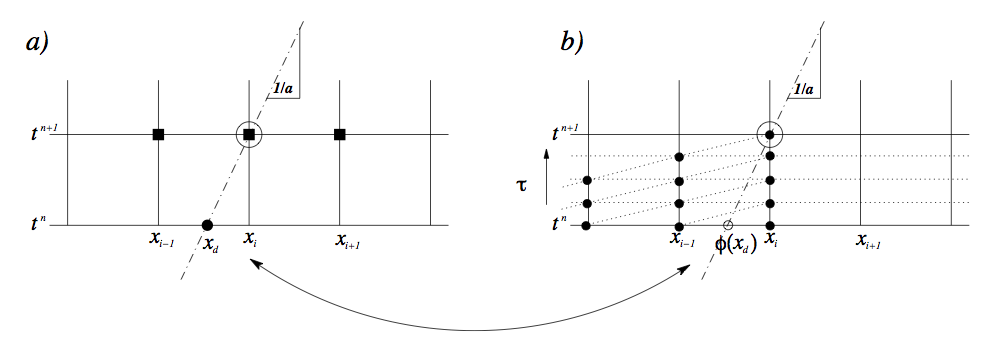
\includegraphics[width=1 \textwidth]{img/substepimage.png}}
   \caption {Schematic representation of the substepping approach. (a)
     Making an explicit time step the hyperbolic solution, travelling
     with a speed $a$, can be understood as being related to the
     solution at point $x_d$ (the departure point). (b) Making smaller
     explicit time steps we can evaluate the solution $\phi(x_d)$ at
     the departure point and then use this value to make a
     semi-Lagrangian discretisation of the implicit components usually
     associated with diffusion.}
\end{figure}


A schematic of the approach can be understood from figure
\ref{fig.substep} where we observe that smaller time steps can be used
for the explicit advection steps whilst a larger overall time step is
adopted for the more expensive implicit solve for the diffusion
operator. More details of the implementation can be found in
\cite{XiShDoKa} and \cite{Sh03}. In the following sections we outline
the parameters that can be used to set up this scheme. Since the
explicit part is advanced using a DG scheme it is necessary to use a
\inltt{Mixed\_CG\_Discontinuous} expansion with this option.

\begin{notebox}
Example of the substepping scheme can be found in the regression tests
directory under
\texttt{\${NEKHOME}/Solver/IncNavierStokesSolver/Tests/} directory. For
exmaple the test cases \texttt{KovaFlow\_SubStep\_2order.xml},
\texttt{Hex\_Kovasnay\_SubStep.xml} and
\texttt{Tet\_Kovasnay\_SubStep.xml}
\end{notebox}

\subsection{Direct solver (coupled approach)}
\label{DirectSolv}
The second approach consists of directly solving the matrix problem
arising from the discretization of the Stokes problem.  The direct
solution of the Stokes system introduces the problem of appropriate
spaces for the velocity and the pressure systems to satisfy the
inf-sup condition and it requires the solution of the full
velocity-pressure system. However, if a discontinuous pressure space
is used then all but the constant mode of the pressure system can be
decoupled from the velocity. When implementing this
approach with a spectral/hp element discretization, the remaining
velocity system may then also be statically condensed to decouple the so
called interior elemental degrees of freedom, reducing the Stokes
problem to a smaller system expressed on the elemental boundaries. The
direct solution of the Stokes problem provides a very natural setting
for the solution of the pressure system which is not easily dealt with
in a splitting scheme. Further, the solution of the full coupled
velocity system allows the introduction of a spatially varying
viscosity, which arise for non-Newtonian flows, with only minor
modifications.

We consider the weak form of the Stokes problem for the velocity field
$boldsymbol{u}=[u,v]^{T}$ and the pressure field $p$:

\begin{subequations}
\begin{equation}
 (\nabla \phi,\nu \nabla \boldsymbol{u}) - (\nabla\cdot\phi,p)=(\phi,\boldsymbol{f})
\end{equation}
\begin{equation}
 (q,\nabla \cdot \boldsymbol{u}) = 0
\end{equation}
\end{subequations}

where the components of $A$,$B$ and $C$ are
$\nabla\phi_b,\nu\nabla\boldsymbol{u_b}$,
$\nabla\phi_b,\nu\nabla\boldsymbol{u_i}$ and
$\nabla\phi_i,\nu\nabla\boldsymbol{u_i}$ and the components $D_b$ and
$D_i$ are $q,\nabla\boldsymbol{u_b}$ and $q,\nabla\boldsymbol{u_i}$.
The indices $b$ and $i$ refer to the degrees of freedom on the
elemental boundary and interior respectively. In constructing the
system we have lumped the contributions form each component of the
velocity field into matrices $A$,$B$ and $C$. However, we note that
for a Newtonian fluid the contribution from each field is
decoupled. Since the interior degrees of freedom of the velocity field
do not overlap, the matrix $C$ is block diagonal and to take advantage
of this structure we can statically condense out the $C$ matrix to
obtain the system:

\begin{equation}
\left[ \begin{array}{ccc}
 A-BC^{-1}B^T & D_b^T-BC^{-1}D_i & 0\\
 D_b-D_i^TC^{-1}B^T & -D_i^TC^{-1}D_i & 0\\
 B^T & D_i & C
 \end{array}\right]
 \left[ \begin{array}{c}
 \boldsymbol{u_b}\\
 p\\
 \boldsymbol{u_i}
 \end{array}\right] =
 \left[ \begin{array}{c}
 \boldsymbol{f_b} - BC^{-1}\boldsymbol{f_i}\\
 -D_i^TC^{-1}\boldsymbol{f_i}\\
 \boldsymbol{f_i}
 \end{array}\right]
 \end{equation}

 To extend the above Stokes solver to an unsteady Navier-Stokes solver
 we first introduce the unsteady term, $\partial
 \boldsymbol{u}/\partial t$, into the Stokes problem.  This has the
 principal effect of modifying the weak Laplacian operator
 $\nabla\phi,\nu\nabla\boldsymbol{u}$] into a weak Helmholtz operator
   $\nabla\phi,\nu\nabla\boldsymbol{u})-\lambda(\phi,\boldsymbol{u}$
   where $\lambda$ depends on the time integration scheme. The second
   modification requires the explicit discretisation of the non-linear
   terms in a similar manner to the splitting scheme and this term is
   then introduced as the forcing term $\boldsymbol{f}$. For more details see \cite{AiSh,ShAi}.

\subsection{Linear Stability Analysis}

Hydrodynamic stability is an important part of fluid-mechanics that has a relevant role in understanding how an unstable flow can evolve into a turbulent state of motion with chaotic three-dimensional vorticity fields and a broad spectrum of small temporal and spatial scales. The essential problems of hydrodynamic stability were recognised and formulated in 19th century, notably by Helmholtz, Kelvin, Rayleigh and Reynolds.

Conventional linear stability assumes a normal representation of the perturbation fields that can be represented as independent wave packets, meaning that the system is self-adjoint. The main aim of the global stability analysis is to evaluate the amplitude of the eigenmodes as time grows and tends to infinity. However, in most industrial applications, it is also interesting to study the behaviour at intermediate states that might affects significantly the functionality and performance of a device. The study of the transient evolution of the perturbations is seen to be strictly related to the non-normality of the linearised Navier-Stokes equations, therefore the normality assumptiong of the system is no longer assumed. The eigenmodes of a non-normal system do not evolve independently and their interaction is responsible for a non-negligible transient growth of the energy. Conventional stability analysis generally does not capture this behaviour, therefore other techniques should be used.

A popular approach to study the hydrodynamic stability of flows consists in performing a direct numerical simulation of the linearised Navier-Stokes equations using iterative methods for computing the solution of the associated eigenproblem. However, since linearly stable flows could show a transient increment of energy, it is necessary to extend this analysis considering the combined effect of the direct and adjoint evolution operators. This phenomenon has noteworthy importance in several engineering applications and it is known as transient growth.

In Nektar++ it is then possible to use the following tools to perform stability analysis:

\begin{itemize}
\item direct stability analysis;
\item adjoint stability analysis;
\item  transient growth analysis;
\end{itemize}

\subsubsection{Direct stability analysis}


The equations that describe the evolution of an infinitesimal disturbance in the flow can be derived decomposing the solution into a basic state $(\mathbf{U}, p)$ and a perturbed state  $\mathbf{U}+\varepsilon \mathbf{u'}$ with $\varepsilon \ll 1$ that both satisfy the Navier-Stokes equations. Substituting into the Navier Stokes equations and considering that the quadratic terms $\mathbf{u'} \cdot \nabla \mathbf{u'}$can be neglected, we obtain the linearised Navier-Stokes equations:

\begin{subequations}
\begin{equation}
  \frac{\partial \mathbf{u'}}{\partial t} + \mathbf{U} \cdot  \nabla \mathbf{u'}+\mathbf{u'} \cdot \nabla \mathbf{U} = -\nabla p + \nu \nabla^2 \mathbf{u'} + \mathbf{f}
\end{equation}

\begin{equation}
\nabla \cdot \mathbf{u'}
\end{equation}

\end{subequations}



The linearised Navier-Stokes equations are identical in form to the non-linear equation, except for the non-linear advection term. Therefore the numerical techniques used for solving Navier-Stokes equations can still be applied as long as the non-linear term is substituted with the linearised one. It is possible to define the linear operator that evolved the perturbation forward in time:

\begin{equation}
   \mathbf{u'}(\mathbf{x},t)=\mathcal{A}(\mathbf{U})\mathbf{u'}(\mathbf{x},0)
\end{equation}

Let us assume that the base flow  $\mathbf{U}$ is steady, then the perturbations are autonomous and we can assume that:

\begin{equation}
   \mathbf{u'}(\mathbf{x},t)=\mathbf{q'}(\mathbf{x})\exp(\lambda t) \quad \mbox{where} \, \lambda=\sigma+i \omega
\end{equation}

Then we obtain the associated eigenproblem:

\begin{equation}
   \mathcal{A}(\mathbf{U})\mathbf{q'}=\lambda \mathbf{q'}
\end{equation}

The dominant eigenvalue determines the behaviour of the flow. If it the real part is positive there exists exponentially growing solutions, conversely if every single eigenvalues has negative real part then the flow is linearly stable. If the real part of the eigenvalue is zero, it is present a bifurcation point.

\subsubsection{Adjoint Stability Analysis}

The adjoint of a linear operator is one of the most important concept in functional analysis and has an it has important role to tackle the transition to turbulence. Let us write the linearised Navier-Stokes equation in a compact form:

\begin{equation}
\mathcal{H}\mathbf{q}=0 \quad \mbox{where} \quad \mathcal{H}=\left( \begin{array}{c|c}
  -\partial_t-(\mathbf{U} \cdot \nabla)+ (\nabla \mathbf{U}) \cdot + \frac{1}{Re} \nabla^2 & -\nabla \\
  \hline
  \nabla \cdot  & 0
   \end{array}
 \right)
 \end{equation}


The adjoint operator $(\mathcal{H}^*$ is defines as:

\begin{equation}
\left \langle \mathcal{H}\mathbf{q}, \mathbf{q} \right \rangle= \left \langle \mathbf{q}, \mathcal{H}^*\mathbf{q}^* \right \rangle
\end{equation}

Integrating by parts and employing the divergence theorem, it is possible to express the adjoint equations:

\begin{subequations}
\begin{equation}
-\frac{\partial \mathbf{u}^*}{\partial t}+(\mathbf{U} \cdot \nabla)\mathbf{u}^*+(\nabla \mathbf{U})^T \cdot \mathbf{u}^*=-\nabla p^*+\frac{1}{Re} \nabla^2 \mathbf{u}
\end{equation}

\begin{equation}
\nabla \cdot \mathbf{u}^*=0
\end{equation}
\end{subequations}

The adjoint fields are in fact related to the concept of \textbf{receptivity}. The value of the adjoint velocity at a point in the flow indicates the response that arises from an unsteady momentum source at that point. The adjoint pressure and the adjoint stream function play instead the same role for mass and vorticity sources respectively. Therefore, the adjoint modes can be seen as a powerful tool to understand where to act in order to ease/inhibit the transition.

\subsubsection{Transient Growth Analysis}

Transient growth  is a phenomenon that occurs when a flow that is linearly stable, but whose perturbations exhibit a non-negligible transient response due to regions of localised convective instabilities. This situation is common in many engineering applications, for example in open flows where the geometry is complex, producing a steep variation of the base flow. Therefore, the main question to answer is if it exists a bounded solution that exhibit large growth before inevitably decaying. Let us introduce a norm to quantify the size of a perturbation. It is physically meaningful to use the total kinetic energy of a perturbation on the domain $\Omega$. This is convenient because it is directly associated with the
standard-$L2$ inner product:

\begin{equation}
\mathcal{A}(\tau)\mathbf{v}=\sigma \mathbf{u}, \quad \left\| \mathbf{u} \right\|=1
\end{equation}


where $\sigma=\left\| \mathbf{u'}(\tau)\right\|$. This is no other
that the singular value decomposition of $\mathcal{A}(\tau)$. The
phenomenology of the transient growth can be explained considering the
non-normality of the linearised Navier-Stokes evolution operator. This
can be simply understood using the simple geometric example showed in
figure \ref{TG}. Let us assume a unit-length vector $\mathbf{f}$
represented in a non-orthogonal basis .This vector is defined as the
difference of the nearly collinear vectors $\mathbf{\Phi_1}$ and
$\mathbf{\Phi_2}$.  With the time progression, the component of these
two vectors decrease respectively by 20\% and 50\%. The vector
$\mathbf{f}$ increases substantially in length before decaying to
zero. Thus, the superposition of decaying non-orthogonal eigenmode can
produce in short term a growth in the norm of the perturbations.


\begin{figure}[!htbp]
\centering
 \label{TG}
 {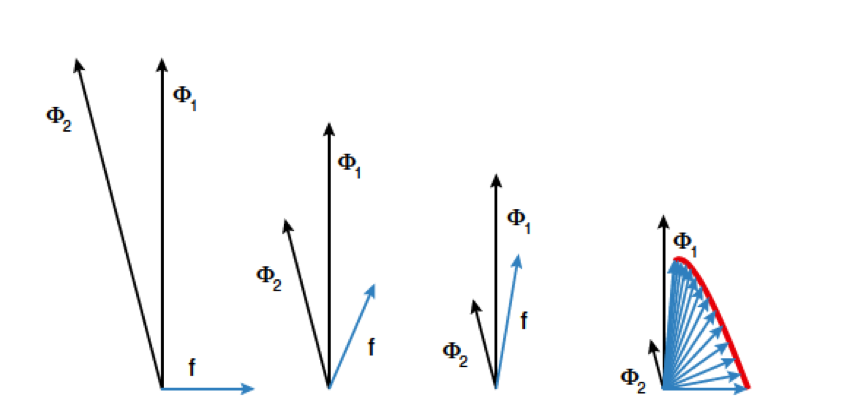
\includegraphics[width=1 \textwidth]{img/transient_growth.png}}
   \caption {Geometric interpretation of the transient growth. Adapted from Schmid, 2007 }
\end{figure}


\subsection{Steady-state solver using Selective Frequency Damping}
\label{SectionSFD}

To compute linear stability analysis, the choice of the base flow,
around which the system will be linearised, is crucial. If one wants
to use the steady-state solution of the Navier-Stokes equations as
base flow, a steady-state solver is implemented in \nekpp. The method
used is the encapsulated formulation of the Selective Frequency
Damping method \cite{JoCoSh14}. Unstable steady base flows can be
obtained with this method. The SFD method is based on the filtering
and control of unstable temporal frequencies within the flow. The time
continuous formulation of the SFD method is
\begin{equation}
\begin{cases}
\dot{q}=NS(q)-\chi (q-\bar{q}), \\
\dot{\bar{q}}=\frac{q-\bar{q}}{\Delta}.
\end{cases}
\label{SFD-General}
\end{equation}
where $q$ represents the problem unknown(s), the dot represents the time derivative, $NS$ represents the Navier-Stokes equations, $\chi \in \mathbb{R}_+$ is the control coefficient, $\bar{q}$ is a filtered version of $q$, and $\Delta \in \mathbb{R}_+ ^*$ is the filter width of a first-order low-pass time filter. The steady-state solution is reached when $q=\bar{q}$.

The convergence of the method towards a steady-state solution depends on the choice of the parameters $\chi$ and $\Delta$. They have to be carefully chosen: if they are too small, the instabilities within the flow can not be damped; but if they are too large, the method may converge extremely slowly. If the dominant eigenvalue of the flow studied is known (and given as input), the algorithm implemented can automatically select parameters that ensure a fast convergence of the SFD method. Most of the time, the dominant eigenvalue is not know, that is why an adaptive algorithm that adapts $\chi$ and $\Delta$ all along the solver execution is also implemented.

Note that this method can not be applied for flows with a pure exponential growth of the instabilities (\textit{e.g.} jet flow within a pipe). In other words, if the frequency of the dominant eigenvalue is zero, then the SFD method is not a suitable tool to obtain a steady-state solution.



\section{Usage}

\begin{lstlisting}[style=BashInputStyle]
IncNavierStokesSolver session.xml
\end{lstlisting}

\section{Session file configuration}

In the following the possible options are shown for the incompressible
Navier-Stokes. The \texttt{Expansion} section for an incompressible flow
simulation can be set as for other solvers regardless of the projection type.
Here an example for a 3D simulation (for 2D simulations the specified fields
would be just \inltt{u,v,p}).

\begin{lstlisting}[style=XMLStyle]
<EXPANSIONS>
  <E COMPOSITE="C[0]" NUMMODES="6" FIELDS="u,v,w,p" TYPE="MODIFIED" />
</EXPANSIONS>
\end{lstlisting}

In case of a simulation using the Direct Solver we need to set
\inltt{FIELDS=u,v} as the pressure expansion order will be automatically set to
fulfil the inf-sup condition. Possible choices for the expansion \inltt{TYPE}
are:
\begin{center}
\footnotesize
\begin{tabular}{lcc}
\toprule
{Basis} & {\texttt{TYPE}} \\
\midrule
\texttt{Modal} & \texttt{MODIFIED} \\
\texttt{Nodal} & \texttt{GLL\_LAGRANGE} \\
\texttt{Nodal SEM} & \texttt{GLL\_LAGRANGE\_SEM} \\
\bottomrule
\end{tabular}
\end{center}

\subsection{Solver Info}
\label{SectionIncNS_SolverInfo}

The following parameters can be specified in the \inltt{SOLVERINFO} section of
the session file:

\begin{itemize}
\item \inltt{EqType}: sets the kind of equations we want to solve on the domain
as:

\begin{lstlisting}[style=XMLStyle]
<I PROPERTY="EQTYPE" VALUE="UnsteadyNavierStokes"/>
\end{lstlisting}

Possible values are:
\begin{center}
\footnotesize
\renewcommand\arraystretch{1.2}
\begin{tabular}{lccccc}
\toprule
{Equations} & {\texttt{EQTYPE}} &{Dim.}&{Projections} & Alg.\\
\midrule
Steady Stokes (SS)& \texttt{SteadyStokes} & All & CG &VCS \\
Steady Oseen (SO) & \texttt{SteadyOseen} & All & CG& DS \\
Unsteady Stokes (US) & \texttt{UnsteadyStokes} & All & CG &VCS \\
Steady Linearised NS (SLNS) & \texttt{SteadyLinearisedNS} & All & CG & DS \\
Unsteady Linearised NS (ULNS) & \texttt{UnsteadyLinearisedNS} & All & CG & VCS,DS \\
Unsteady NS (UNS) & \texttt{UnsteadyNavierStokes} & All & CG,CG-DG & VCS \\
\bottomrule
\end{tabular}
\end{center}


\item \inltt{SolverType}: sets the scheme we want to use to solve the set of
equations as
\begin{lstlisting}[style=XMLStyle]
<I PROPERTY="SolverType"  VALUE="VelocityCorrectionScheme"/>
\end{lstlisting}

Possible values are:
\begin{center}
\footnotesize
\begin{tabular}{lcccc}
\toprule
{Algorithm} & {\texttt{SolverType}} &{Dimensions}&{Projections} \\
\midrule
Velocity Correction Scheme & \texttt{VelocityCorrectionScheme} & 2D, Quasi-3D, 3D & CG, CG-DG\\
Direct solver & \texttt{CoupledLinearisedNS} & 2D, Quasi-3D, 3D &CG\\
\bottomrule
\end{tabular}
\end{center}

\item \inltt{Driver}: this specifies the type of problem to be solved:
\begin{center}
\footnotesize
\begin{tabular}{lcccc}
\toprule
{Driver} & {Description} &{Dimensions}&{Projections} \\
\midrule
\texttt{Standard} & Time integration of the equations & All & CG, DG \\
\texttt{SteadyState} & Steady-state solver (see Sec. \ref{SectionSFD})  & All & CG, DG \\
\bottomrule
\end{tabular}
\end{center}

\item \inltt{Projection}: sets the Galerkin projection type as
\begin{lstlisting}[style=XMLStyle]
<I PROPERTY="Projection" VALUE="Continuous"/>
\end{lstlisting}

Possible values are:
\begin{center}
\footnotesize
\begin{tabular}{lccccc}
\toprule
{Galerkin Projection} & \texttt{Projection} &{Dimensions}&{Equations}&{Algorithms} \\
\midrule
Continuous (CG)&  \texttt{Continuous} & All & All & All \\
Discontinuous (DG) & \texttt{DisContinuous} & All &...&...\\
Mixed CG and DG (CG-DG) & \texttt{Mixed\_CG\_Discontinuous} & 2D,3D & just UNS & VCS-substepping \\
\bottomrule
\end{tabular}
\end{center}


\item \inltt{TimeIntegrationMethod}:  sets the time integration method as
\begin{lstlisting}[style=XMLStyle]
<I PROPERTY="TimeIntegrationMethod" VALUE="IMEXOrder2"/>
\end{lstlisting}

Possible values are
\begin{center}
\footnotesize
\begin{tabular}{lcccccc}
\toprule
{Time-Integration Method} & \texttt{TimeIntegrationMethod} &{Dimensions}&{Equations}&Projections\\
\midrule
IMEX Order 1 & \texttt{IMEXOrder1} & all & US, UNS &  CG \\
IMEX Order 2 & \texttt{IMEXOrder2} & all & US, UNS &  CG \\
IMEX Order 3 & \texttt{IMEXOrder3} & all & US, UNS & CG \\
Backward Euler & \texttt{BackwardEuler} & all & US, UNS &  CG-DG \\
BDF Order 1 & \texttt{BDFImplicitOrder1} & all & US, UNS & CG-DG \\
BDF Order 2 & \texttt{BDFImplicitOrder2} & all & US, UNS & CG-DG \\
\bottomrule
\end{tabular}
\end{center}

\item \inltt{Extrapolation}: Specify the extrapolation method
  (standard or substetping) to be used in velocity correction
  scheme. Essentially this activates the sub-stepping routine which
  requires the mixed CG-DG projection
  
\begin{lstlisting}[style=XMLStyle]
<I PROPERTY="Extrapolation" VALUE="SubStepping"/>
\end{lstlisting}

Possible values are \inltt{SubStepping} or \inltt{Standard} with ``Standard'' being the default value if nothing is specifiied. 

\item \inltt{SubStepIntScheme}: choose the substep DG time integration
  scheme so that a different order schems can be used as compared to
  the overal time integraiton scheme.
\begin{lstlisting}[style=XMLStyle]
<I PROPERTY="SubStepIntScheme" VALUE="RungeKutta2\_ImprovedEuler"/>
\end{lstlisting}

Possible values are
\begin{center}
\footnotesize
\begin{tabular}{lc}
\toprule
{Time-Integration Method} & \texttt{SubStepIntScheme} \\
\midrule
Forward Euler & \texttt{ForwardEuler}  \\
RK 2          & \texttt{RungeKutta2\_ImprovedEuler}  \\
\bottomrule
\end{tabular}
\end{center}

This option is useful if you wish to use an overall scheme that is
first order accurate for example with
TimeIntegrationMethod as BDFImplicitOrder1 but using a second order
RungeKutta2\_ImprovedEuler for greater stability in the substep.

\item \inltt{GlobalSysSoln}: sets the approach we use to solve the the linear
systems of the type $Ax=b$ appearing in the solution steps, such as the Poisson
equation for the pressure in the splitting-scheme. It can be set as

\begin{lstlisting}[style=XMLStyle]
<I PROPERTY="GlobalSysSoln" VALUE="IterativeStaticCond"/>
\end{lstlisting}

Possible values are
\begin{center}
\footnotesize
\begin{tabular}{lccc}
\toprule
{System solution} & \texttt{GlobalSysSoln} &{Parallel}\\
\midrule
Direct Solver (DS) & \texttt{DirectFull} & just quasi-3D \\
DS with Static Condensation  & \texttt{DirectStaticCond} & just Quasi-3D \\
DS with Multilevel Static Condensation & \texttt{DirectMultiLevelStaticCond} & just Quasi-3D \\
 Iterative Solver (IS) & \texttt{IterativeFull} & just Quasi-3D \\
IS with Static Condensation  & \texttt{IterativeStaticCond} & quasi-3D \\
IS with Multilevel Static Condensation & \texttt{IterativeMultiLevelStaticCond} & quasi-3D \\
\bottomrule
\end{tabular}
\end{center}

Default values are \inltt{DirectMultiLevelStaticCond} in serial and
\inltt{IterativeStaticCond} in parallel.

\item \inltt{SmoothAdvection}: activates a stabilization technique which smooths
the advection term using the pressure inverse mass matrix. It can be used just in combination with nodal expansion basis for efficiency reasons.

\begin{lstlisting}[style=XMLStyle]
<I PROPERTY="SmoothAdvection" VALUE="True"/>
\end{lstlisting}


\item \inltt{SpectralVanishingViscosity}: activates a stabilization technique
which increases the viscosity on the modes with the highest frequencies.
\begin{lstlisting}[style=XMLStyle]
<I PROPERTY="SpectralVanishingViscosity" VALUE="True"/>
\end{lstlisting}

In a Quasi-3D simulation, this will affect both the Fourier and the spectral/hp expansions.
To activate them independently, use \inltt{SpectralVanishingViscositySpectralHP} 
and \inltt{SpectralVanishingViscosityHomo1D}.

\item \inltt{DEALIASING}: activates the 3/2 padding rule on the advection term
of a Quasi-3D simulation.
\begin{lstlisting}[style=XMLStyle]
<I PROPERTY="DEALIASING" VALUE="ON"/>
\end{lstlisting}


\item \inltt{SPECTRALHPDEALIASING}: activates the spectral/hp dealiasing to
stabilize the simulation. This method is based on the work of Kirby and Sherwin [7].
\begin{lstlisting}[style=XMLStyle]
<I PROPERTY="SPECTRALHPDEALIASING" VALUE="True" />
\end{lstlisting}

\end{itemize}


\subsection{Parameters}
The following parameters can be specified in the \inltt{PARAMETERS} section of
the session file:

\begin{itemize}
\item \inltt{TimeStep}: sets the time-step for the integration in time formula
\item \inltt{NumSteps}: sets the number of time-steps
\item \inltt{Kinvis}: sets the cinematic viscosity coefficient formula
\item \inltt{SubStepCFL}: sets the CFL safety limit for the sub-stepping algorithm (default value = 0.5)
\item \inltt{MinSubSteps}: perform a minimum number of substeps in sub-stepping algorithm (default is 1)
\item \inltt{MaxSubSteps}: perform a maxmimum  number of substeps in sub-stepping algorithm otherwise exit (default is 100)
\item \inltt{SVVCutoffRatio}: sets the ratio of Fourier frequency not affected by the SVV technique (default value = 0.75, i.e. the first 75\% of frequency are not damped)
\item \inltt{SVVDiffCoeff}: sets the SVV diffusion coefficient (default value = 0.1)
\end{itemize}

\subsection{Forcing}
\subsubsection{MovingBody}

\begin{notebox}
This force type is only supported for the Quasi-3D incompressible Navier-Stokes solver.
\end{notebox}

This force type allows the user to solve the interaction system of an incompressible fluid flowing past a flexible moving bodies ~\cite{NeKa97}. By this forcing function, one can eliminate the difficulty of moving mesh by using body-fitted coordinates, so that an additional acceleration term(i.e., forcing term) is introduced to the momentum equations by the non-inertial transform from the deformed and moving coordinate system to non-deformed and stationary one.

\begin{lstlisting}[style=XMLStyle]
<FORCE TYPE="MovingBody">
</FORCE>
\end{lstlisting}

Available options of the motion type for the moving body include free, constrained and forced vibrations, which can be specified in the \inltt{SOLVERINFO} section. The free type of motion allows the body to move in both streamwise and crossflow directions, while the constrained type limits the motion only in the crossflow direction. For the forced type, the vibration profiles of the body should be specified as a given function or read from input file in \inltt{MovingBody} section. here an example,

\begin{lstlisting}[style=XMLStyle]
<SOLVERINFO>
    <I PROPERTY="EQTYPE"    VALUE="UnsteadyNavierStokes" />
    <I PROPERTY="SolverType"    VALUE="VelocityCorrectionScheme" />
    <I PROPERTY="EvolutionOperator"    VALUE="SkewSymmetric" />
    <I PROPERTY="Projection"    VALUE="Galerkin" />
    <I PROPERTY="GlobalSysSoln"    VALUE="DirectStaticCond"/>
    <I PROPERTY="TimeIntegrationMethod"    VALUE="IMEXOrder2" />
    <I PROPERTY="HOMOGENEOUS"    VALUE="1D"/>
    <I PROPERTY="USEFFT"    VALUE="FFTW"/>
    <I PROPERTY="VibrationType"    VALUE="FREE"/>
</SOLVERINFO>
\end{lstlisting}

A moving body type boundary condition should be specified in \inltt{BOUNDARYCONDITIONS} for the velocities on the moving body,

\begin{lstlisting}[style=XMLStyle]
<BOUNDARYCONDITIONS>
    <REGION REF="0">
        <D VAR="u" USERDEFINEDTYPE="MovingBody" VALUE="0" />
        <D VAR="v" USERDEFINEDTYPE="MovingBody" VALUE="0" />
        <D VAR="w" VALUE="0" />
        <N VAR="p" USERDEFINEDTYPE="H" VALUE="0" />
     </REGION>
</BOUNDARYCONDITIONS>
\end{lstlisting}

For the simulation of low mass ratio, there is an option to activate fictitious mass method for stabilizing explicit coupling between the fluid solver and structural dynamic solver. Here we need to specify the values of fictitious mass and damping in \inltt{PARAMETERS}, for example,

\begin{lstlisting}[style=XMLStyle]
<SOLVERINFO>
    <I PROPERTY="FictitiousMassMethod"    VALUE="True"/>
</SOLVERINFO>
<PARAMETERS>
    <P> FictDamp      = 1000    </P>
    <P> FictMass       = 1.5       </P>
</PARAMETERS>
\end{lstlisting}

A filter calles as \inltt{MovingBody} is encapsulated in this module to evaluate the aerodynamic forces along the moving body surface. The
forces for each computational plane are projected along the Cartesian axes and the pressure and viscous
contributions are computed in each direction.

The following parameters are supported:

\begin{center}
  \begin{tabularx}{0.99\textwidth}{lllX}
    \toprule
    \textbf{Option name} & \textbf{Required} & \textbf{Default} &
    \textbf{Description} \\
    \midrule
    \inltt{OutputFile}      & \xmark   & \inltt{session} &
    Prefix of the output filename to which the forces are written.\\
    \inltt{Frequency}       & \xmark   & 1 &
    Number of timesteps after which output is written.\\
    \inltt{Boundary}        & \cmark   & - &
    Boundary surfaces on which the forces are to be evaluated.\\
    \bottomrule
  \end{tabularx}
\end{center}

To enable the filter, add the following to the \inltt{FORCE} tag::

\begin{lstlisting}[style=XMLStyle]
  <FORCE TYPE="MovingBody">
      <PARAM NAME="OutputFile">DragLift.frc</PARAM>
      <PARAM NAME="OutputFrequency">10</PARAM>
      <PARAM NAME="Boundary"> B[0] </PARAM>
  </FORCE>
\end{lstlisting}

During the execution a file named \inltt{DragLift.frc} will be created and the
value of the aerodynamic forces on boundary 0, defined in the
\inltt{GEOMETRY} section, will be output every 10 time steps.evaluates the aerodynamic forces along the moving body surface. The
forces for each computational plane are projected along the Cartesian axes and the pressure and viscous contributions are computed in each direction.

Also, to use this module a \inltt{MAPPING} needs to be specified, as described in section \ref{sec:mapping}. In the case of free and constrained motion presented here, the functions defined by the mapping act as initial conditions. Also, when using the MovingBody forcing, it is not necessary to set the \inltt{TIMEDEPENDENT} property of the mapping. 

\section{Stability analysis Session file configuration}
\label{SecStabFile}
The type of equation which is to be solved is specified through the \inltt
{EqType} option in the session file. This can be set to any of the following:

\begin{center}
\footnotesize
\begin{tabular}{lc}
\toprule
{Equation to solve}  \\
\midrule
$\frac{\partial\mathbf{u'}}{\partial t} +\mathcal{L}(\mathbf{U},\mathbf{u'})=-\nabla p+\nu \nabla^2 \mathbf{u'}$\\
\bottomrule
\end{tabular}
\end{center}


\begin{center}
\footnotesize
\begin{tabular}{lccccc}
\toprule
{Equation Type} & {Dimensions} &{Projections} &{Algorithms} \\
\midrule
UnsteadyNavierStokes & 2D, Quasi-3D& Continuous &VCS,DS\\
\bottomrule
\end{tabular}
\end{center}

\subsection{Solver Info}
\label{SectionIncNS_SolverInfo_Stab}

\begin{itemize}
\item \inltt{Eqtype}:  sets the type of equation to solve, according to the
table above.
\item \inltt{TimeIntegrationMethod}: the following types of time integration methods have been tested with each solver:
\begin{center}
\footnotesize
\begin{tabular}{lccccc}
\toprule
{} & {Explicit} &{Diagonally Implicit} &{IMEX} & {Implicit} \\
\midrule
\texttt{UnsteadyNavierStokes} & X & &X & \\
\bottomrule
\end{tabular}
\end{center}

\item \inltt{Projection}: the Galerkin projection used may be either
\begin{itemize}
\item \inltt{Continuous}: for a C0-continuous Galerkin (CG) projection;
\item \inltt{Discontinuous}: for a discontinous Galerkin (DG) projection.
\end{itemize}

\item \inltt{EvolutionOperator}:
\begin{itemize}
\item \inltt{Nonlinear} (non-linear Navier-Stokes equations).
\item \inltt{Direct} (linearised Navier-Stokes equations).
\item \inltt{Adjoint} (adjoint Navier-Stokes equations).
\item \inltt{TransientGrowth} ((transient growth evolution operator).
\end{itemize}

\item \inltt{Driver}: specifies  the type of problem to be solved:
   \begin{itemize}
    \item \inltt{Standard} (time integration of the equations)
    \item \inltt{ModifiedArnoldi} (computations of the leading eigenvalues and eigenmodes using modified Arnoldi method)
    \item \inltt{Arpack} (computations of eigenvalues/eigenmodes using Implicitly Restarted Arnoldi Method (ARPACK) ).
    \end{itemize}

\item \inltt{ArpackProblemType}: types of eigenvalues to be computed (for Driver Arpack only)
\begin{itemize}
\item \inltt{LargestMag} (eigenvalues with largest magnitude).
\item \inltt{SmallestMag} (eigenvalues with smallest magnitude).
\item \inltt{LargestReal} (eigenvalues with largest real part).
\item \inltt{SmallestReal} (eigenvalues with smallest real part).
\item \inltt{LargestImag} (eigenvalues with largest imaginary part).
\item \inltt{SmallestIma} (eigenvalues with smallest imaginary part ).
\end{itemize}

\item \inltt{Homogeneous}: specifies the Fourier expansion in a third direction (optional)
\begin{itemize}
\item \inltt{1D} (Fourier spectral method in z-direction).
\end{itemize}
\item \inltt{ModeType}: this specifies the type of the quasi-3D problem to be solved.
\begin{itemize}
\item \inltt{MultipleMode} (stability analysis with multiple modes).
\item \inltt{SingleMode} (BiGlobal Stability Analysis: full-complex mode).
\item \inltt{HalfMode} (BiGlobal Stability Analysis: half-complex mode u.Re v.Re w.Im p.Re).
\end{itemize}
\end{itemize}


\subsection{Parameters}
The following parameters can be specified in the \texttt{PARAMETERS} section of the session file:

\begin{itemize}
\item \inltt{Re}: sets the Reynolds number
\item \inltt{Kinvis}: sets the kinematic viscosity $\nu$.
\item \inltt{kdim}: sets the dimension of the Krylov subspace $\kappa$. Can be used in: \inltt{ModifiedArnoldi} and \inltt{Arpack}. Default value: 16.
\item \inltt{evtol}: sets the tolerance of the eigenvalues. Can be used in: \item \inltt{imagShift}: provide an imaginary shift to the direct sovler eigenvalue problem by the specified value. 
ltt{ModifiedArnoldi} and \inltt{Arpack}. Default value: $10^{-6}$.
\item \inltt{nits}: sets the maximum number of iterations. Can be used in: \inltt{ModifiedArnoldi} and \inltt{Arpack}. Default value: 500.
\item \inltt{LZ}:  sets the length in the spanswise direction $L_z$. Can be used in \inltt{Homogeneous} set to \inltt{1D}. Default value: 1.
\item \inltt{HomModesZ}: sets the number of planes in the homogeneous directions. Can be used in \inltt{Homogeneous} set to \inltt{1D} and \inltt{ModeType} set to \inltt{MultipleModes}.
\item \inltt{N\_slices}: sets the number of temporal slices for Floquet stability analysis.
\item \inltt{period}: sets the periodicity of the base flow.
\item \inltt{realShift}: provide a real shift to the direct sovler eigenvalue problem by the specified value. 
\end{itemize}

\subsection{Functions}
When using the direct solver for stability analysis it is necessary to specify a Forcing function ``StabilityCoupledLNS'' in the form:
\begin{lstlisting}[style=XMLStyle]
<FORCING>
   <FORCE TYPE="StabilityCoupledLNS">
   </FORCE>
</FORCING>
\end{lstlisting}

This is required since we need to tell the solver to use the existing
field as a forcing function to the direct matrix inverse as part of
the Arnoldi iteration.


\begin{notebox}
Examples of the set up of the direct solver stability analysis (and
other incompressible Navier-Stokes solvers) can be found in the
regression test directory
\inlsh{NEKTAR/solvers/IncNavierStokesSolver/Tests}. See for example the files
\inlsh{PPF\_R15000\_ModifiedArnoldi\_Shift.tst} and \inlsh{PPF\_R15000\_3D.xml}
noting that some parameters are specified in the .tst files.
\end{notebox}

\section{Steady-state solver Session file configuration}
\label{SectionSFD_XML}

In this section, we detail how to use the steady-state solver (that
implements the selective frequency damping method, see
Sec. \ref{SectionSFD}).  Two cases are detailed here: the execution of
the classical SFD method and the \textit{adaptive} SFD method, where
the control coefficient $\chi$ and the filter width $\Delta$ of the
SFD method are updated all along the solver execution. For the second
case, the parameters of the SFD method do not need to be defined by
the user (they will be automatically calculated all along the solver
execution) but several session files must be defined in a very
specific way.

\subsection{Execution of the classical steady-state solver}

\subsubsection{Solver Info}

The definition of \inltt{Eqtype}, \inltt{TimeIntegrationMethod} and
\inltt{Projection} is similar as what is explained in
\ref{SectionIncNS_SolverInfo_Stab}. The use of the steady-state solver
is enforced through the definition of the \inltt{Driver} which has to be
\inltt{SteadyState}. \inltt{EvolutionOperator} does not need to be
defined to run the unadapted SFD method (by default, it is set to
\inltt{Nonlinear}).

\subsubsection{Parameters}

The following parameters can be specified in the \texttt{PARAMETERS} section of the session file:

\begin{itemize}
%\item \inltt{Re}: sets the Reynolds number
\item \inltt{Kinvis}: sets the kinematic viscosity $\nu$. It is typically $1/Re$ if both the characteristic velocity and characteristic length are chosen to be 1. 
\item \inltt{ControlCoeff}: sets the control coefficient $\chi$ of the SFD method. Default value: 1.
\item \inltt{FilterWidth}: sets the filter width $\Delta$ of the SFD method. Default value: 2.
\item \inltt{GrowthRateEV} and \inltt{FrequencyEV}: if the growth rate and the frequency of the dominant eigenvalue are known, they can be given given as input and the code will automatically select the optimum parameters $\chi$ and $\Delta$ (and overwrite the values of \inltt{ControlCoeff} and \inltt{GrowthRateEV} that may be given in the session file)
\item \inltt{TOL}: sets the tolerance of the SFD method. The code will run until $||q-\bar{q}||_{inf}<TOL$.  Default value: $10^{-8}$.
\end{itemize}

Note that for the steady-state solver, the parameter \inltt{NumSteps} is not taken into account. The solver will run until a steady-state solution is found and not for a pre-defined number of time steps.

\subsection{Execution of the adaptive steady-state solver}

Running the adaptive selective frequency damping method requires to set up the session files in a very specific manner. First, the \inltt{Geometry} section must be in a separated archive file. If the test case studied is called "Session", the mesh file must be called \inlsh{Session.xml.gz} (the linux command "gzip" can be used to obtain this file).

The requirements for the file \inlsh{Session.xml} are similar as for the ones for the classical SFD method. The \inltt{Geometry} section being removed and placed in \inlsh{Session.xml.gz}. This file defines the properties of the nonlinear problem solved (\textit{i.e.} the flow for which we want a steady-state). Also, the \inltt{SOLVERINFO} section must contain the line:
\begin{lstlisting}[style=XMLStyle]
<I PROPERTY="EvolutionOperator" VALUE="AdaptiveSFD" />
\end{lstlisting}

The adaptive SFD method used is coupled with a stability analysis method. Then \inltt{kdim}, \inltt{nvec}, \inltt{evtol} and \inltt{nits} should be defined into the \inltt{PARAMETERS} section of \inlsh{Session.xml}. If not, these parameters will take the default values presented in Sec. \ref{SecStabFile}.

The goal of running the stability analysis is to evaluate the dominant eigenvalue of a ``partially converged'' steady base flow. This approximation is then used by the steady-state solver to select a control coefficient $\chi$ and a filter width $\Delta$ then ensure a fast convergence towards a steady-state solution.

To define the linear stability problem, another file, that must be called \inlsh{Session\_LinNS.xml}, has to be defined. This file \textbf{must be an exact copy/paste of} \inlsh{Session.xml}, only three things have to be modified:
\begin{enumerate}
\item The boundary conditions must be modified to be homogeneous (\textit{i.e.} equal to zero) at all inflow boundaries.
\item A non-zero function \inltt{InitialConditions} has to be defined.
\item A random function \inltt{BaseFlow} has to be defined (it will be overwritten all along the solver execution). We recommend it to be a copy of \inltt{InitialConditions}.
\end{enumerate}

Once these three files (the  \inltt{Geometry} in \inlsh{Session.xml.gz}, the nonlinear problem definition in \inlsh{Session.xml} and the homogeneous linear problem in \inlsh{Session\_LinNS.xml}) are correctly defined, the adaptive SFD method must be executed using:

\begin{lstlisting}[style=BashInputStyle]
IncNavierStokesSolver Session.xml.gz Session.xml
\end{lstlisting}


\section{Coordinate transformations Session file configuration}\label{sec:mapping}

This section describes how to include a coordinate transformation
to the solution of the incompressible Navier-Stokes equations.
In some cases, this approach allows a slightly deformed geometry to
be mapped into a geometry with a homogeneous direction, which can be treated
using a quasi-3D method. It is also useful for problems with a moving body,
 where otherwise a moving mesh would have to be employed.
 
\subsection{Solver Info}

To activate the mapping technique, \inltt{SolverType} needs to be set as:
\begin{lstlisting}[style=XMLStyle]
<I PROPERTY="SolverType" VALUE="VCSMapping" />
\end{lstlisting}
Also, there are other optional properties in the \inltt{SolverInfo} section:
\begin{lstlisting}[style=XMLStyle]
<I PROPERTY="MappingImplicitPressure" VALUE="TRUE"/> <!-- Default = FALSE -->
<I PROPERTY="MappingImplicitViscous" VALUE="TRUE"/>  <!-- Default = FALSE -->

<I PROPERTY="MappingNeglectViscous" VALUE="FALSE"/>  <!-- Default = FALSE -->
\end{lstlisting}
the first two options determine if the pressure and viscous terms resulting from the
coordinate transformation are treated implicitly using an iterative procedure. If the last
option is set to true, the viscous terms in the mapping are not computed. This leads to a
faster solution, but the effect on the results need to be determined for the specific case. 
 By default, all mapping terms are computed and treated explicitly.
 
\subsection{Parameters}

When treating the mapping terms implicitly, the following parameters can be set:
\begin{lstlisting}[style=XMLStyle]
<P> MappingPressureTolerance    = 1e-8  </P>  <!-- Default = 1e-12  -->
<P> MappingViscousTolerance     = 1e-8  </P>  <!-- Default = 1e-12  -->
<P> MappingPressureRelaxation   = 0.9   </P>  <!-- Default = 1.0    -->
<P> MappingViscousRelaxation    = 0.9   </P>  <!-- Default = 1.0    -->
\end{lstlisting}
They determine the tolerance of the iterative solution of the equations, 
and a relaxation parameter which can improve the numerical stability of the method.

\subsection{Mapping}

The particular transformation employed is specified by:
\begin{lstlisting}[style=XMLStyle]
<MAPPING TYPE="XYofZ">
    <COORDS>Mapping</COORDS>
    <VEL>MappingVel</VEL>
    <TIMEDEPENDENT>True</TIMEDEPENDENT> <!-- Default is False -->
</MAPPING>
\end{lstlisting}
where \inltt{TIMEDEPENDENT} indicates if the transformation varies 
with time.

The available values for \inltt{TYPE}, and the transformations they represent, 
are:
\begin{center}
  \begin{tabular}{llll}
    \toprule
    Mapping type & $\bar{x}$ & $\bar{y}$ & $\bar{z}$ \\
    \midrule
    \inltt{Translation} &  $x +f(t)$  & $y + g(t)$ & $z + h(t)$   \\
    \inltt{XofZ} &  $x + f(z,t)$  & $y$ & $z$   \\
    \inltt{XofXZ} &  $f(x,z,t)$  & $y$ & $z$   \\
    \inltt{XYofZ} &  $x + f(z,t)$  & $y + g(z,t)$ & $z$   \\
    \inltt{XYofXY} &  $f(x,y,t)$  & $g(x,y,t)$ & $z$   \\
    \inltt{General} &  $f(x,y,z,t)$  & $g(x,y,z,t)$ & $h(x,y,z,t)$   \\      
    \bottomrule
  \end{tabular}
\end{center}
where $(\bar{x},\bar{y},\bar{z})$ are the Cartesian (physical) coordinates and 
$(x,y,z)$ are the transformed coordinates. Note that for quasi-3D problems, the
$z$ coordinate cannot be transformed.

\subsection{Functions}

The function \inltt{COORDS} (and \inltt{VEL} for time dependent mappings)
 indicated in the \inltt{MAPPING} section need to be defined, for example as:
\begin{lstlisting}[style=XMLStyle]
        <FUNCTION NAME="Mapping">
            <E VAR="x" VALUE="x + cos(PI*z)" />
            <E VAR="y" VALUE="y + cos(2*PI*t)" />
        </FUNCTION>
        
        <FUNCTION NAME="MappingVel">
            <E VAR="vx" VALUE="0.0" />
            <E VAR="vy" VALUE="-1.0*2*PI*sin(2*PI*t)" />
        </FUNCTION>
\end{lstlisting} 
the transformation defined by these functions need to be valid 
(non-zero Jacobian). By default, any component of \inltt{COORDS} that
is not specified is taken as a trivial transformation, e.g. $\bar{x} = x$,
 and any velocity not specified is considered to be zero.
 
\subsection{Boundary conditions}

In case of a time-dependent mapping, a moving body boundary condition
is available: 
\begin{lstlisting}[style=XMLStyle]
<BOUNDARYCONDITIONS>
    <REGION REF="0">
        <D VAR="u" USERDEFINEDTYPE="MovingBody" VALUE="0" />
        <D VAR="v" USERDEFINEDTYPE="MovingBody" VALUE="0" />
        <D VAR="w" VALUE="0" />
        <N VAR="p" USERDEFINEDTYPE="H" VALUE="0" />
     </REGION>
</BOUNDARYCONDITIONS>
\end{lstlisting}
When using the \inltt{MovingBody} boundary condition, the Dirichlet condition
is relative to the boundary, while the regular Dirichlet boundary condition
is taken in an absolute sense. 

All Dirichlet boundary conditions are specified in the Cartesian (physical) space,
 and are automatically transformed to the computational frame of reference. 
 
\begin{notebox}
Examples of the use of mappings can be found in the test directory
\inlsh{NEKTAR/solvers/IncNavierStokesSolver/Tests}. See for example the files
\inlsh{KovaFlow\_3DH1D\_P8\_16modes\_Mapping-implicit.xml} and \inlsh{CylFlow\_Mov\_mapping.xml}.
\end{notebox}

\section{Adaptive polynomial order Session file configuration}
\label{SectionDriverAdaptive}

An adaptive polynomial order procedure is available for 2D and
Quasi-3D simulations.  This procedure consists of the following steps:
\begin{itemize}
\item Advance the equations for a determined number of time steps
\item Use the sensor defined in equation \ref{eq:sensor} to 
estimate an error measure (the variable used in the sensor can be specified).
 The error is defined here as the square of the sensor.  
\item Use the error to determine if the order in each element should be
increased by one, decreased by one, or left unaltered.
\item Project the solution in each element to the new polynomial order and use it as an
initial condition to restart the equation, repeating all steps a given number of times.
\end{itemize}

It is important to note that restarting the simulation after the refinement can be an
expensive operation (in a typical case 200 times the cost of a single time step). Therefore, the number
of steps between successive refinements needs to be carefully chosen, since if this value is too 
low the procedure becomes inefficient, while if it is too high the refinement might not capture
accurately structures that are convected by the flow.  

\subsection{Solver Info}

The use of the adaptive polynomial order procedure
is enforced through the definition of the \inltt{Driver} which has to be
\inltt{Adaptive}.

\subsection{Parameters}

The following parameters can be specified in the \texttt{PARAMETERS} section of the session file:

\begin{itemize}
\item \inltt{NumSteps}: when using the adaptive order procedure, this parameter determines
 the number of time steps between successive refinements.
\item \inltt{NumRuns}: this parameter defines the number of times the sequence of solving
 the equation and refining is performed. Therefore,
  the total number of time steps in the simulation is $NumSteps \times NumRuns$.
\item \inltt{AdaptiveMaxModes}: sets the maximum number of modes (in each direction)
 that can be used in an element during the adaptive procedure. The solution will not be
  refined beyond this point, even if the error is higher than the tolerance. Default value: 12.
\item \inltt{AdaptiveMinModes}: sets the minimal number of modes (in each direction)
 that can be used in an element during the adaptive procedure. Default value: 4.
\item \inltt{AdaptiveUpperTolerance}: defines a constant tolerance. The polynomial order
 in an element is increased whenever the error is higher than this value. This can be replaced
  by a spatially-varying function, as described below. Default value: $10^{-6}$.
\item \inltt{AdaptiveLowerinModes}: defines a constant tolerance. The polynomial order in an
 element is decreased whenever the error is lower than this value. This can also be replaced
  by a spatially-varying function. Default value: $10^{-8}$.
\item \inltt{AdaptiveSensorVariable}: integer defining which variable will be considered when calculating
 the error. For example, if this parameter is set to $1$ in the Incompressible Navier-Stokes Solver,
  the error will be estimated using the $v$ velocity. Default value: $0$.
\end{itemize}

\subsection{Functions}

Spatially varying tolerances can be specified by defining the
functions \inltt{AdaptiveLowerinModes} and/or
\inltt{AdaptiveUpperTolerance}. In this case, the tolerance in an
element is taken as the average of the function in the quadrature
points of the element. If these functions are defined, the values set
for the tolerances in the \texttt{PARAMETERS} section are ignored.

\section{Advecting extra passive scalar fields}

In some cases, it might be useful to advect passive scalar fields with the velocity obtained from the
solution of the Navier-Stokes equation. For example, in study of mass transfer or heat transfer problems
where getting analytical expression for advection velocity is not possible, the transport (advection-diffusion)
equation needs to be solved along with the Navier-Stokes equation to get the scalar concentration or
temperature distribution in the flow field.

In the input file, the extra field variables that are being advected need to be defined after the variables
representing the velocity components. The pressure needs to be at the end of the list. For example, for
a 2D simulation the expansions and variables would be defined as

\begin{lstlisting}[style=XMLStyle]
<EXPANSIONS>
    <E COMPOSITE="C[0]" NUMMODES="5" FIELDS="u,v,c1,c2,p" TYPE="MODIFIED" />
</EXPANSIONS>

<VARIABLES>
    <V ID="0"> u  </V>
    <V ID="1"> v  </V>
    <V ID="2"> c1 </V>
    <V ID="3"> c2 </V>
    <V ID="4"> p  </V>
</VARIABLES>
\end{lstlisting}
where u, v are the velocity components, c1 and c2 are extra fields that are being advected and p is the pressure.

In addition, diffusion coefficients for each extra variable can be specified by adding a function
\inltt{DiffusionCoefficient}
\begin{lstlisting}[style=XMLStyle]
<FUNCTION NAME="DiffusionCoefficient">
    <E VAR="c1" VALUE="0.1" />
    <E VAR="c2" VALUE="0.01" />
</FUNCTION>
\end{lstlisting}

Boundary conditions for the extra fields are set up in the same way as the velocity and pressure
\begin{lstlisting}[style=XMLStyle]
<BOUNDARYCONDITIONS>
  <REGION REF="0">
    <D VAR="u"  VALUE="0" />
    <D VAR="v"  VALUE="0" />
    <D VAR="c1" VALUE="1" />
    <D VAR="c2" VALUE="0" />
    <N VAR="p"  USERDEFINEDTYPE="H" VALUE="0" />
  </REGION>
</BOUNDARYCONDITIONS>
\end{lstlisting}

It should be noted that if the diffusion coefficient is too small, the transport equation becomes advection dominated.
This leads to small grid spacing required to resolve all physical scales associated with the transport equation
(the ratio of resolution required for transport to Navier Stokes equation scales with $Sc^{3/4}$, where $Sc$ is the
Schmidt number = kinematic viscosity/diffusion coefficient). Hence, small diffusion coefficient might lead to spurious
oscillations if the mesh spacing is not small enough.

\section{Examples}

\subsection{Kovasznay Flow 2D}
\label{s:incns:kovasznay2D}
This example demonstrates the use of the velocity correction
\hyperref{VCSscheme}{velocity correction scheme} to solve the 2D Kovasznay flow
at Reynolds number $Re=40$.
% %
In the following we will numerically solve for the two dimensional velocity and
pressure fields with steady boundary conditions.

\subsubsection{Input file}
The input for this example is given in the example file
\inlsh{KovaFlow\_m8.xml}. The mesh consists of 12 quadrilateral elements.

We will use a 7th-order polynomial expansions ($N=8$ modes) using the
modified Legendre basis and therefore require the following expansion
definition.
\begin{lstlisting}[style=XMLStyle]
<EXPANSIONS>
  <E COMPOSITE="C[0]" NUMMODES="6" FIELDS="u,v,p" TYPE="MODIFIED" />
</EXPANSIONS>
\end{lstlisting}

We next specify the solver information for our problem. In particular, we select
the velocity correction scheme formulation, using a continuous Galerkin
projection. For this scheme, an implicit-explicit ime-integration scheme must be
used and we choose one of second order.
\begin{lstlisting}[style=XMLStyle]
<SOLVERINFO>
  <I PROPERTY="EQTYPE" VALUE="UnsteadyNavierStokes" />
  <I PROPERTY="SolverType" VALUE="VelocityCorrectionScheme" />
  <I PROPERTY="AdvectionForm" VALUE="Convective" />
  <I PROPERTY="Projection" VALUE="Galerkin" />
  <I PROPERTY="TimeIntegrationMethod" VALUE="IMEXOrder2" />
</SOLVERINFO>
\end{lstlisting}

The key parameters are listed below. Since the problem is unsteady we prescribe
the time step and the total number of time steps. We also know the required
Reynolds number, but we must prescribe the kinematic viscosity to the solver. We
first define a \emph{dummy} parameter for the Reynolds number, and then define
the kinematic viscosity as the inverse of this. The value of $\lambda$ is used
when defining the boundary conditions and exact solution. Note that \inltt{PI}
is a pre-defined constant.

\begin{lstlisting}[style=XMLStyle]
<PARAMETERS>
  <P> TimeStep      = 0.001  </P>
  <P> NumSteps      = 100    </P>
  <P> Re            = 40     </P>
  <P> Kinvis        = 1/Re   </P>
  <P> LAMBDA        = 0.5*Re-sqrt(0.25*Re*Re+4*PI*PI)</P>
</PARAMETERS>
\end{lstlisting}

We choose to impose a mixture of boundary condition types as defined below.

\begin{lstlisting}[style=XMLStyle]
<BOUNDARYCONDITIONS>
    <REGION REF="0">
        <D VAR="u" VALUE="1-exp(LAMBDA*x)*cos(2*PI*y)" />
        <D VAR="v" VALUE="(LAMBDA/2/PI)*exp(LAMBDA*x)*sin(2*PI*y)" />
        <N VAR="p" USERDEFINEDTYPE="H" VALUE="0" />
    </REGION>
    <REGION REF="1">
        <D VAR="u" VALUE="1-exp(LAMBDA*x)*cos(2*PI*y)" />
        <D VAR="v" VALUE="(LAMBDA/2/PI)*exp(LAMBDA*x)*sin(2*PI*y)" />
        <D VAR="p" VALUE="0.5*(1-exp(2*LAMBDA*x))" />
    </REGION>
    <REGION REF="2">
        <N VAR="u" VALUE="0" />
        <D VAR="v" VALUE="0" />
        <N VAR="p" VALUE="0" />
    </REGION>
</BOUNDARYCONDITIONS>
\end{lstlisting}

Initial conditions are obtained from the file KovaFlow\_m8.rst, which is
a \nekpp field file. This is the output of an earlier simulation, renamed with
the extension \inltt{rst} to avoid being overwritten, and is used in this case
to reduce the integration time necessary to obtain the steady flow.
\begin{lstlisting}[style=XMLStyle]
<FUNCTION NAME="InitialConditions">
    <F FILE="KovaFlow_m8.rst" />
</FUNCTION>
\end{lstlisting}
Note the use of the \inltt{F} tag to indicate the use of a file. In contrast,
the exact solution is prescribed using analytic expressions which requires the
use of the \inltt{E} tag.
\begin{lstlisting}[style=XMLStyle]
<FUNCTION NAME="ExactSolution">
    <E VAR="u" VALUE="1-exp(LAMBDA*x)*cos(2*PI*y)" />
    <E VAR="v" VALUE="(LAMBDA/2/PI)*exp(LAMBDA*x)*sin(2*PI*y)" />
    <E VAR="p" VALUE="0.5*(1-exp(2*LAMBDA*x))" />
</FUNCTION>
\end{lstlisting}

\subsubsection{Running the simulation}
Launch the simulation using the following command
\begin{lstlisting}[style=BashInputStyle]
IncNavierStokesSolver KovaFlow_m8.xml
\end{lstlisting}
After completing the prescribed 100 time-steps, the difference between the
computed solution and the exact solution will be displayed. The actual mantissas
may vary slightly, but the overall magnitude should be as shown.
\begin{lstlisting}[style=BashInputStyle]
L 2 error (variable u) : 3.75296e-07
L inf error (variable u) : 5.13518e-07
L 2 error (variable v) : 1.68897e-06
L inf error (variable v) : 2.23918e-06
L 2 error (variable p) : 1.46078e-05
L inf error (variable p) : 5.18682e-05
\end{lstlisting}

The output of the simulation is written to \inlsh{KovaFlow\_m8.fld}. This can be
visualised by converting it to a visualisation format. For example, to use
ParaView, convert the output into VTK format using the
\hyperref{s:utilities:fieldconvert}{FieldConvert} utility.
\begin{lstlisting}[style=BashInputStyle]
FieldConvert KovaFlow.xml KovaFlow.fld KovaFlow.vtu
\end{lstlisting}
The result should look similar to that shown in Figure~\ref{f:incns:kovaflow}.

\begin{figure}
\begin{center}
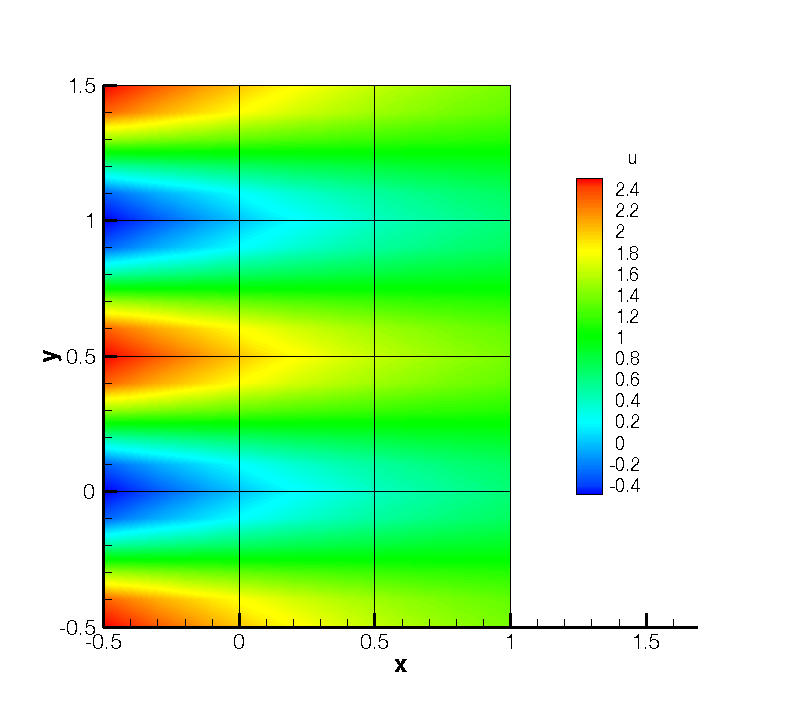
\includegraphics[width=7cm]{img/KF2DCVP8.png}
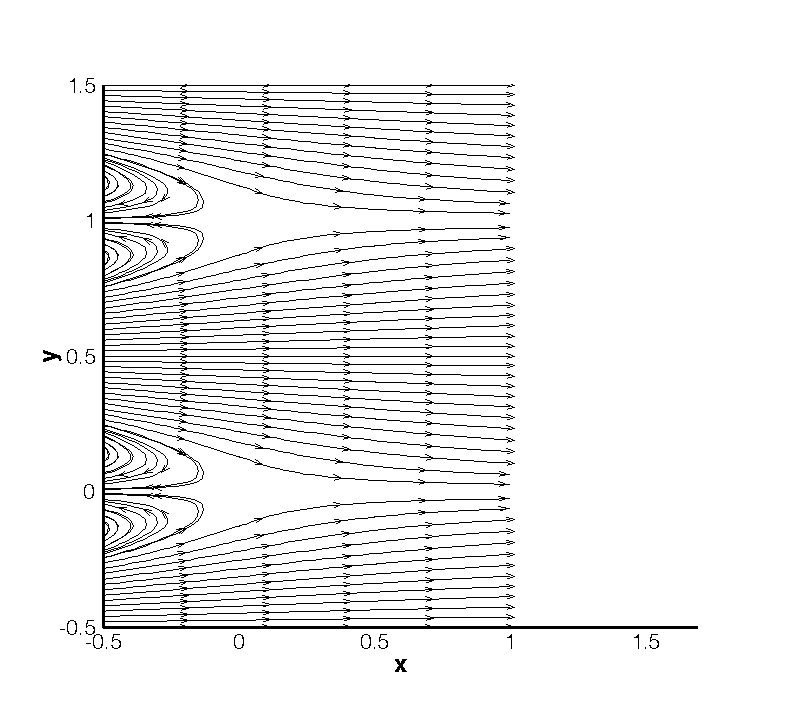
\includegraphics[width=7cm]{img/KF2DCVP8SL.png}
\caption{Velocity profiles for the Kovasznay Flow (2D).}
\label{f:incns:kovaflow}
\end{center}
\end{figure}

\subsection{Kovasznay Flow 2D using high-order outflow boundary conditions}
\label{s:incns:kovasznay2D_HOBC}
In this example, we solve the same case of 2D Kovasznay flow on
severely-truncated computational domain but using a high-order outflow
boundary condition, which is much more accurate and robust for
unbounded flows~\cite{DoKa14}. The solver information and parameters
used here are similar to the previous one. What only we need to modify
in the input file is just the boundary condition type upon the outlet
region shown as below
\begin{lstlisting}[style=XMLStyle]
<BOUNDARYCONDITIONS>
    <REGION REF="0">
        <D VAR="u" VALUE="1-exp(KovLam*x)*cos(2*PI*y)" />
        <D VAR="v" VALUE="(KovLam/2/PI)*exp(KovLam*x)*sin(2*PI*y)" />
        <N VAR="p" USERDEFINEDTYPE="H" VALUE="0" />
    </REGION>
    <REGION REF="1">
        <N VAR="u" USERDEFINEDTYPE="HOutflow" 
              VALUE="-Kinvis*KovLam*exp(KovLam*x)*cos(2*PI*y) 
		- 0.5*(1-exp(2*KovLam*x))-0.5*(((1-exp(KovLam*x)*cos(2*PI*y))
		*(1-exp(KovLam*x)*cos(2*PI*y))+(KovLam/(2*PI)*exp(KovLam*x)
		*sin(2*PI*y))*(KovLam/(2*PI)*exp(KovLam*x)*sin(2*PI*y))))
		*(0.5*(1.0-tanh((1-exp(KovLam*x)*cos(2*PI*y))*20)))" />
        <N VAR="v" USERDEFINEDTYPE="HOutflow" 
              VALUE="Kinvis*KovLam*KovLam/(2*PI)*exp(KovLam*x)*sin(2*PI*y)" />
        <D VAR="p" USERDEFINEDTYPE="HOutflow" 
              VALUE="-Kinvis*KovLam*exp(KovLam*x)*cos(2*PI*y)
		- 0.5*(1-exp(2*KovLam*x)) -0.5*(((1-exp(KovLam*x)*cos(2*PI*y))
		*(1-exp(KovLam*x)*cos(2*PI*y))+(KovLam/(2*PI)*exp(KovLam*x)
		*sin(2*PI*y))*(KovLam/(2*PI)*exp(KovLam*x)*sin(2*PI*y))))
		*(0.5*(1.0-tanh((1-exp(KovLam*x)*cos(2*PI*y))*20)))" />
    </REGION>
    <REGION REF="2">
        <N VAR="u" VALUE="0" />
        <D VAR="v" VALUE="0" />
        <N VAR="p" VALUE="0" />
    </REGION>
</BOUNDARYCONDITIONS>
\end{lstlisting} 
We note that in this example the ``VALUE'' property is set based on
the analytic solution but this is not typically known and so often a
VALUE of zero will be specified.

Instead of loading an initial condition from a specified file, we initialized the flow fields in this example by using following expressions
\begin{lstlisting}[style=XMLStyle]
<FUNCTION NAME="InitialConditions">
    <E VAR="u" VALUE="(1-exp(KovLam*x)*cos(2*PI*y))" />
    <E VAR="v" VALUE="(KovLam/(2*PI))*exp(KovLam*x)*sin(2*PI*y)" />
    <E VAR="p" VALUE="0.5*(1-exp(2*KovLam*x))" />
</FUNCTION>
\end{lstlisting}
\subsubsection{Running the simulation}
We then launch the simulation by the same solver as that in the previous example
\begin{lstlisting}[style=BashInputStyle]
IncNavierStokesSolver KovaFlow_m8_short_HOBC.xml
\end{lstlisting} 
 The solution with errors displayed as below
\begin{lstlisting}[style=BashInputStyle]
L 2 error (variable u) : 2.51953e-08
L inf error (variable u) : 9.56014e-09
L 2 error (variable v) : 1.10694e-08
L inf error (variable v) : 9.47464e-08
L 2 error (variable p) : 5.59175e-08
L inf error (variable p) : 2.93085e-07
\end{lstlisting}

The physical solution visualized in velocity profiles is also illustrated in 
Figure~\ref{f:incns:kovaflow2d_hobc}.

\begin{figure}
\begin{center}
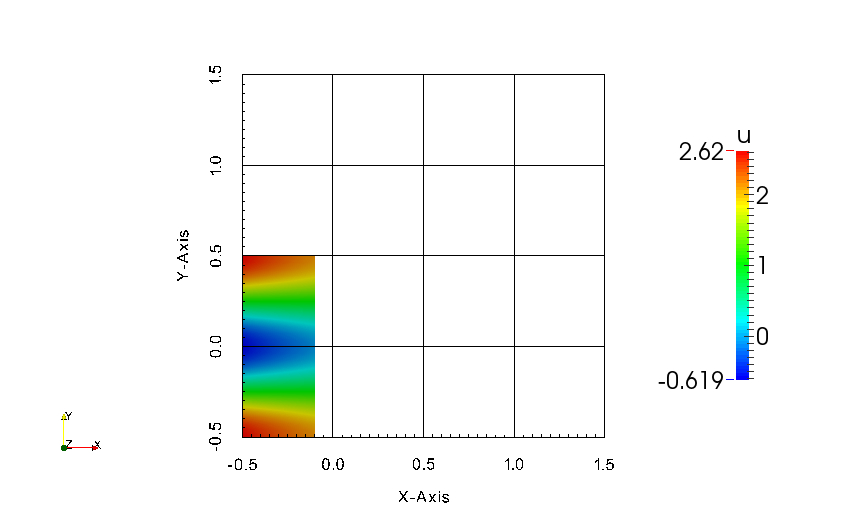
\includegraphics[width=7cm]{img/KF2DCVP8HOBC_U.png}
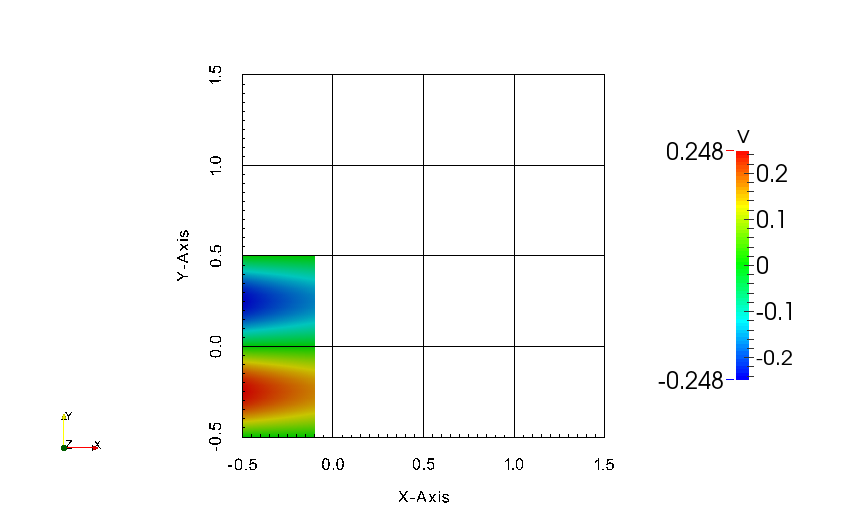
\includegraphics[width=7cm]{img/KF2DCVP8HOBC_V.png}
\caption{Velocity profiles for the Kovasznay Flow in truncated domain (2D).}
\label{f:incns:kovaflow2d_hobc}
\end{center}
\end{figure}

\subsection{Steady Kovasznay Oseen Flow using the direct solver}
\label{s:incns:kovasznay2Ddirect}
In this example, we instead compute the steadhy Kovasznay Oseen flow
using the direct solver. In contrast to the velocity correction scheme in which
we time-step the solution to the final time, the direct solver computes the
solution with a single solve.

\subsubsection{Input file}
We can begin with the same input file as for the previous example, but with the
following modifications. For reference, the modified version is provided in the
example \inlsh{Oseen\_m8.xml}.

In the solver information, we must instead select the
Steady-Oseen equation type and choose to use the coupled linearised
Navier-Stokes
\begin{lstlisting}[style=XMLStyle]
<I PROPERTY="EQTYPE" VALUE="SteadyOseen" />
<I PROPERTY="SolverType" VALUE="CoupledLinearisedNS" />
\end{lstlisting}

\begin{notebox}
Since we are using a coupled system, we are not solving for the pressure. We
should therefore remove all references to the variable \inltt{p} in the session.
In particular, it should be removed from the \inltt{EXPANSIONS},
\inltt{VARIABLES}, \inltt{BOUNDARYCONDITIONS} and \inltt{FUNCTIONS} sections of
the file.
\end{notebox}

Instead of loading an initial condition from file, we can simply prescribe a
zero field.
\begin{lstlisting}[style=XMLStyle]
<FUNCTION NAME="InitialConditions">
    <E VAR="u" VALUE="0" />
    <E VAR="v" VALUE="0" />
</FUNCTION>
\end{lstlisting}

We must also provide an advection velocity.
\begin{lstlisting}[style=XMLStyle]
<FUNCTION NAME="AdvectionVelocity">
    <E VAR="u" VALUE="(1-exp(-LAMBDA*x)*cos(2*PI*y))" />
    <E VAR="v" VALUE="(-LAMBDA/(2*PI))*exp(-LAMBDA*x)*sin(2*PI*y)" />
</FUNCTION>
\end{lstlisting}

\subsubsection{Running the simulation}
Run the simulation using
\begin{lstlisting}[style=BashInputStyle]
IncNavierStokesSolver Oseen_m8.xml
\end{lstlisting}

The resulting flow field should match the solution from the previous example.


\subsection{Laminar Channel Flow 2D}
\label{s:incns:LaminarChannelFlow2D}
In this example, we will simulate the flow through a channel at Reynolds number
1 with fixed boundary conditions.

\subsubsection{Input file}
The input file for this example is given in \inltt{ChanFlow\_m3\_SKS.xml}. The
geometry is a square channel with height and length $D=1$, discretised using
four quadrilateral elements. We use a quadratic expansion order, which is
sufficient to capture the quadratic flow profile. In this example, we choose to
use the skew-symmetric form of the advection term. This is chosen in the solver
information section:
\begin{lstlisting}[style=XMLStyle]
<I PROPERTY="EvolutionOperator" VALUE="SkewSymmetric" />
\end{lstlisting}
A first-order time integration scheme is used and we set the time-step and
number of time integration steps in the parameters section. We also prescribe
the kinematic viscosity $\nu = 1/Re = 1$.

Boundary conditions are defined on the walls (region 0) and at the inflow
(regions 1) as Dirichlet for the velocity field and as high-order for the
pressure. At the outflow the velocity is left free using Neumann boundary
conditions and the pressure is pinned to zero.
\begin{lstlisting}[style=XMLStyle]
<BOUNDARYCONDITIONS>
    <REGION REF="0">
        <D VAR="u" VALUE="0" />
        <D VAR="v" VALUE="0" />
        <N VAR="p" USERDEFINEDTYPE="H" VALUE="0" />
    </REGION>
    <REGION REF="1">
        <D VAR="u" VALUE="y*(1-y)" />
        <D VAR="v" VALUE="0" />
        <N VAR="p" USERDEFINEDTYPE="H" VALUE="0" />
    </REGION>
    <REGION REF="2">
        <N VAR="u" VALUE="0" />
        <N VAR="v" VALUE="0" />
        <D VAR="p" VALUE="0" />
    </REGION>
</BOUNDARYCONDITIONS>
\end{lstlisting}

Initial conditions are set to zero. The exact solution is a parabolic profile
with a pressure gradient dependent on the Reynolds number. This is defined to
allow verification of the calculation.
\begin{lstlisting}[style=XMLStyle]
<FUNCTION NAME="ExactSolution">
    <E VAR="u" VALUE="y*(1-y)" />
    <E VAR="v" VALUE="0" />
    <E VAR="p" VALUE="-2*Kinvis*(x-1)" />
</FUNCTION>
\end{lstlisting}

\subsubsection{Running the solver}
\begin{lstlisting}[style=BashInputStyle]
IncNaverStokesSolver ChanFlow_m3_SKS.xml
\end{lstlisting}

The error in the solution should be displayed and be close to machine precision
\begin{lstlisting}[style=BashInputStyle]
L 2 error (variable u) : 4.75179e-16
L inf error (variable u) : 3.30291e-15
L 2 error (variable v) : 1.12523e-16
L inf error (variable v) : 3.32197e-16
L 2 error (variable p) : 1.12766e-14
L inf error (variable p) : 7.77156e-14
\end{lstlisting}

The solution should look similar to that shown in
Figure~\ref{f:incns:laminar2d}.

\begin{figure}
\begin{center}
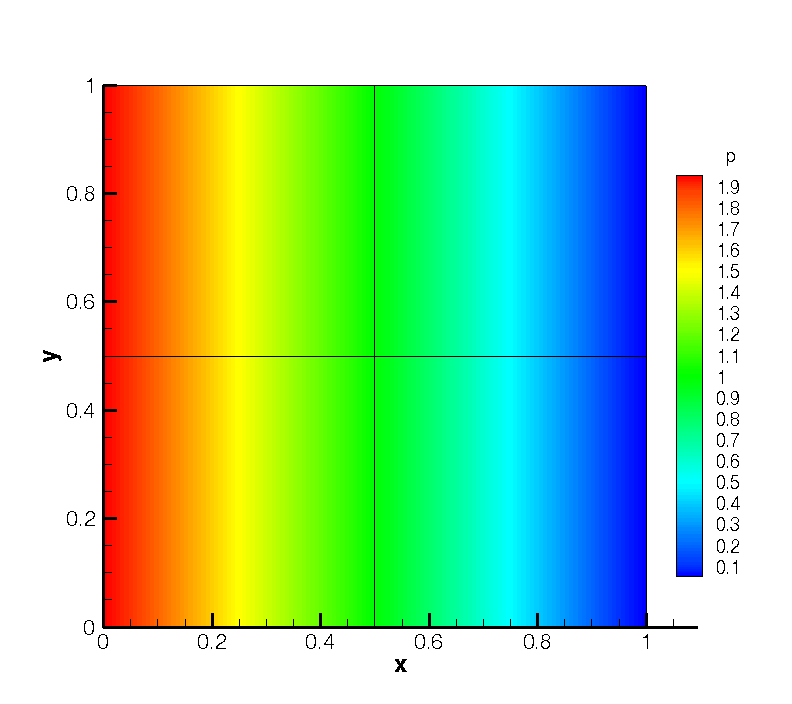
\includegraphics[width=7cm]{img/CF2DSKP3PR.png}
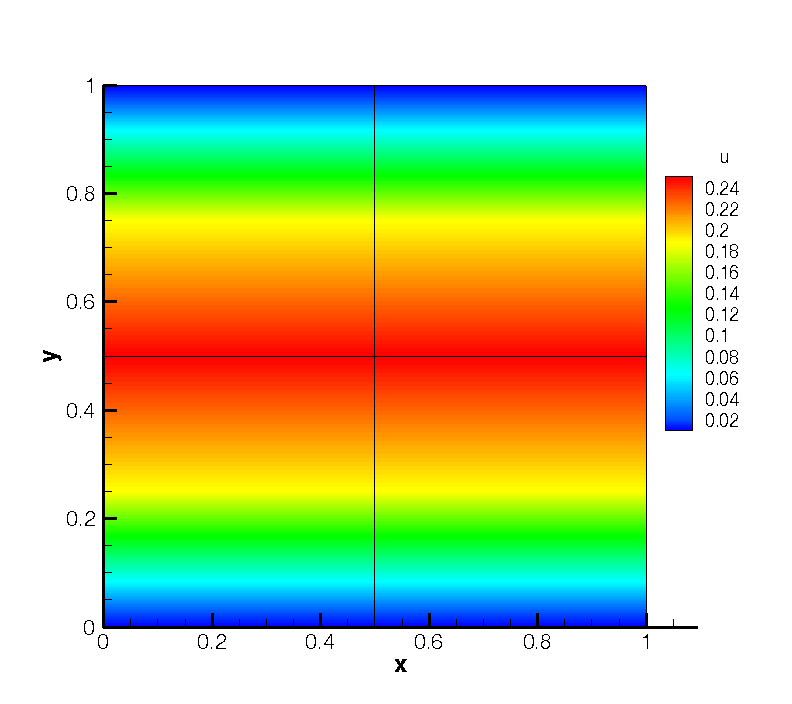
\includegraphics[width=7cm]{img/CF2DSKP3.png}
\caption{Pressure and velocity profiles for the laminar channel flow (2D).}
\label{f:incns:laminar2d}
\end{center}
\end{figure}



\subsection{Laminar Channel Flow 3D}
We now solve the incompressible Navier-Stokes equations on a three-dimensional
domain. In particular, we solver the three-dimensional equivalent of the
previous example. We will also solve the problem in parallel.

\begin{notebox}
In order to run the example, you must have a version of \nekpp compiled with
MPI. This is the case for the packaged binary distributions.
\end{notebox}

\subsubsection{Input file}
The input file for this example is given in \inlsh{Tet\_channel\_m8\_par.xml}.
In this example we use tetrahedral elements, indicated by the \inltt{A} element
tags in the geometry section. All dimensions have length $D=1$. We will use a
7th-order polynomial expansion. Since we now have three dimensions, and
therefore three velocity components, the expansions section is now
\begin{lstlisting}[style=XMLStyle]
<EXPANSIONS>
  <E COMPOSITE="C[0]" NUMMODES="8" FIELDS="u,v,w,p" TYPE="MODIFIED" />
</EXPANSIONS>
\end{lstlisting}
The solver information and parameters are similar to the previous example.
Boundary conditions must now be defined on the six faces of the domain. Flow is
prescribed in the z-direction through imposing a Poiseulle profile on the inlet
and side walls. The outlet is zero-Neumann and top and bottom faces impose
zero-Dirichlet conditions.
\begin{lstlisting}[style=XMLStyle]
<BOUNDARYREGIONS>
    <B ID="0"> C[1] </B>    <!-- Inlet -->
    <B ID="1"> C[6] </B>    <!-- Outlet -->
    <B ID="2"> C[2] </B>    <!-- Wall -->
    <B ID="3"> C[3] </B>    <!-- Wall left -->
    <B ID="4"> C[4] </B>    <!-- Wall -->
    <B ID="5"> C[5] </B>    <!-- Wall right -->
</BOUNDARYREGIONS>

<BOUNDARYCONDITIONS>
    <REGION REF="0">
        <D VAR="u" VALUE="0" />
        <D VAR="v" VALUE="0" />
        <D VAR="w" VALUE="y*(1-y)" />
        <N VAR="p" USERDEFINEDTYPE="H" VALUE="0" />
    </REGION>
    <REGION REF="1">
        <N VAR="u" VALUE="0" />
        <N VAR="v" VALUE="0" />
        <N VAR="w" VALUE="0" />
        <D VAR="p" VALUE="0" />
    </REGION>
    <REGION REF="2">
        <D VAR="u" VALUE="0" />
        <D VAR="v" VALUE="0" />
        <D VAR="w" VALUE="0" />
        <N VAR="p" USERDEFINEDTYPE="H" VALUE="0" />
    </REGION>
    <REGION REF="3">
        <D VAR="u" VALUE="0" />
        <D VAR="v" VALUE="0" />
        <D VAR="w" VALUE="y*(1-y)" />
        <N VAR="p" USERDEFINEDTYPE="H" VALUE="0" />
    </REGION>
    <REGION REF="4">
        <D VAR="u" VALUE="0" />
        <D VAR="v" VALUE="0" />
        <D VAR="w" VALUE="0" />
        <N VAR="p" USERDEFINEDTYPE="H" VALUE="0" />
    </REGION>
    <REGION REF="5">
        <D VAR="u" VALUE="0" />
        <D VAR="v" VALUE="0" />
        <D VAR="w" VALUE="y*(1-y)" />
        <N VAR="p" USERDEFINEDTYPE="H" VALUE="0" />
    </REGION>
</BOUNDARYCONDITIONS>
\end{lstlisting}

Initial conditions and exact solutions are also prescribed.

\subsubsection{Running the solver}
To run the solver in parallel, we use the \inltt{mpirun} command.
\begin{lstlisting}[style=BashInputStyle]
mpirun -np 2 IncNaverStokesSolver Tet_channel_m8_par.xml
\end{lstlisting}

The expected results are shown in Figure~\ref{f:incns:laminar3d}.

\begin{figure}
\begin{center}
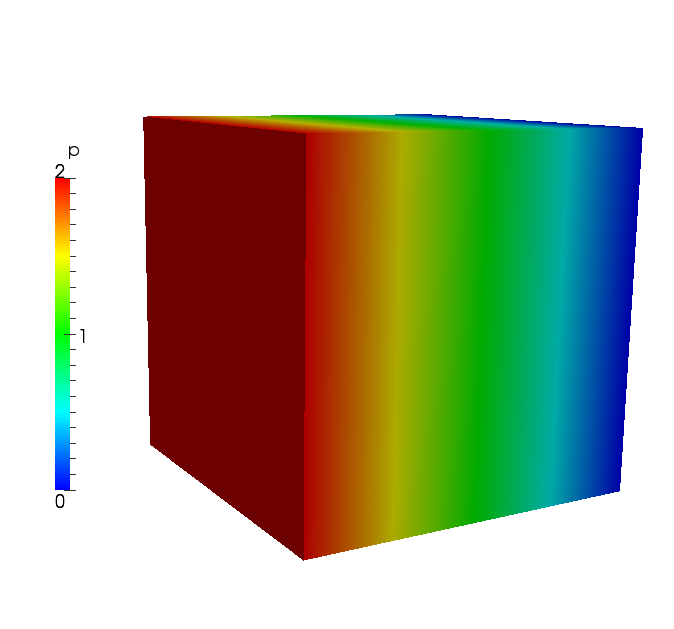
\includegraphics[width=7cm]{img/CF3DP8PR.png}
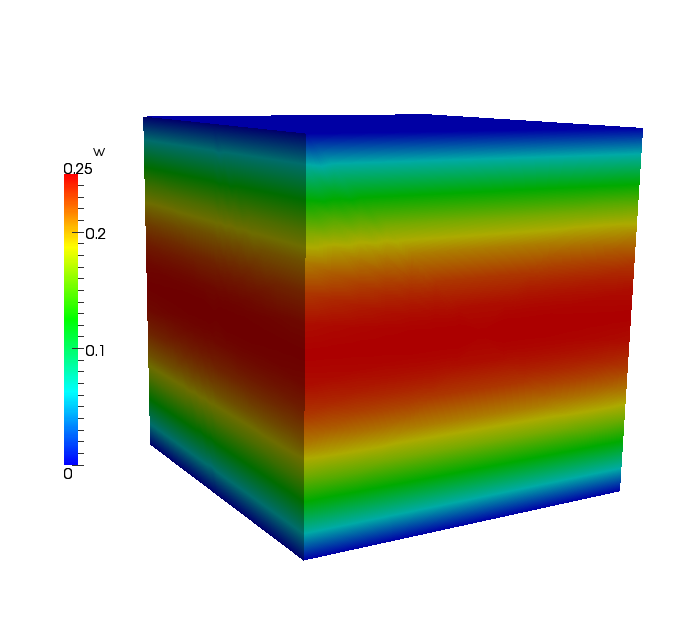
\includegraphics[width=7cm]{img/CF3DP8.png}
\caption{Pressure and velocity profiles for the laminar channel flow (full 3D).}
\label{f:incns:laminar3d}
\end{center}
\end{figure}


\subsection{Laminar Channel Flow Quasi-3D}
For domains where at least one direction is geometrically homogeneous, a more
efficient discretisation is to use a pure spectral discretisation, such as a
Fourier expansion, in these directions. We use this approach to solve the same
problem as in the previous example. We reuse the two-dimensional spectral/hp
element mesh from the \hyperref{s:incns:LaminarChannelFlow2D}{2D laminar flow
example} and couple this with a Fourier expansion in the third component.

\subsubsection{Input file}
The input file for this example is \inlsh{ChanFlow\_3DH1D\_MVM.xml}. We indicate
that we are coupling the spectral/hp element domain with a pure spectral
expansion using the following solver information
\begin{lstlisting}[style=XMLStyle]
<I PROPERTY="HOMOGENEOUS" VALUE="1D"/>
\end{lstlisting}
We must also specify parameters to describe the particular spectral expansion
\begin{lstlisting}[style=XMLStyle]
<P> HomModesZ     = 20       </P>
<P> LZ            = 1.0      </P>
\end{lstlisting}
The parameter \inltt{HomModesZ} specifies the number of Fourier modes to use in
the homogeneous direction. The \inltt{LZ} parameter specifies the physical
length of the domain in that direction.

\newsavebox\incnsFFTWnote
\begin{lrbox}{\incnsFFTWnote}\begin{minipage}{0.8\linewidth}
\begin{lstlisting}[style=XMLStyle]
<I PROPERTY="USEFFT" VALUE="FFTW"/>
\end{lstlisting}
\end{minipage}
\end{lrbox}
\begin{notebox}
This example uses an in-built Fourier transform routine. Alternatively, one can
use the FFTW library to perform Fourier transforms which typically offers
improved performance. This is enabled using the following solver information
\noindent\usebox\incnsFFTWnote
\end{notebox}

As with the \hyperref{s:incns:LaminarChannelFlow2D}{2D case}, the spectral/hp
element mesh consists of four quadrilateral elements with a second-order
polynomial expansion. Since our domain is three-dimensional we have to now
include the third velocity component
\begin{lstlisting}[style=XMLStyle]
<E COMPOSITE="C[0]" NUMMODES="3" FIELDS="u,v,w,p" TYPE="MODIFIED" />
\end{lstlisting}
The remaining parameters and solver information is similar to previous examples.

Boundary conditions are specified as for the two-dimensional case (except with
the addition of the third velocity component) since the side walls are now
implicitly periodic. The initial conditions and exact solution are prescribed as
for the fully three-dimensional case.

\subsubsection{Running the solver}
\begin{lstlisting}[style=BashInputStyle]
IncNaverStokesSolver ChanFlow_3DH1D_MVM.xml
\end{lstlisting}
The results can be post-processed and should match those of the fully
three-dimensional case as shown in Figure~\ref{f:incns:laminar3d}.



\subsection{Turbulent Channel Flow}
In this example we model turbulence in a three-dimensional square channel at a
Reynolds number of 2000.

\begin{notebox}
This example requires the FFTW Fast-Fourier transform library to be selected
when compiling Nektar++.
\end{notebox}

\subsubsection{Input file}
The input file for this example is \inlsh{TurbChFl\_3DH1D.xml}. The geometry
makes used of the homogeneous extension discussed in the previous example. The
channel has height $D=2$ and length $L=4\pi$ and is discretised using quadratic
quadrilateral elements in the spectral/hp element plane and a Fourier basis in
the third coordinate direction. The elements are non-uniformly distributed so as
to best capture the flow features with fewest degrees of freedom and is shown in
Figure~\ref{f:incns:turbchanmesh}.

\begin{figure}
\begin{center}
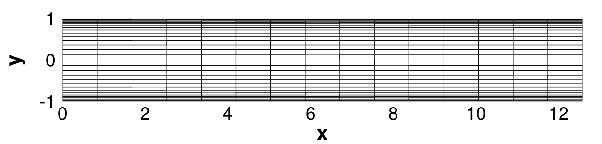
\includegraphics[width=10cm]{img/ChanMesh.png}
\caption{Mesh used for the turbulent channel flow.}
\label{f:incns:turbchanmesh}
\end{center}
\end{figure}

The spanwise length of the channel is set using the \inltt{LZ} parameter and
discretised with 32 Fourier modes by setting the value of \inltt{HomModesZ}.
\begin{lstlisting}[style=XMLStyle]
<P> HomModesZ     = 32          </P>
<P> LZ            = 4*PI/3     </P>
\end{lstlisting}
A second-order IMEX scheme is used for time-integration scheme is used with a
time-step of 0.0001. The length of the simulation is 1 time-unit (10,000 steps).

Periodicity is naturally enforced in the spanwise direction, so boundary
conditions need only be provided for the upper and lower walls, inlet and
outlet as denoted by the following \inltt{BOUNDARYREGIONS}.
\begin{lstlisting}[style=XmlStyle]
<BOUNDARYREGIONS>
  <B ID="0"> C[1] </B> //walls
  <B ID="1"> C[2] </B> //inflow
  <B ID="2"> C[3] </B> //outflow
</BOUNDARYREGIONS>
\end{lstlisting}
In this example, we will use a body force to drive the flow and so, in addition
to the spanwise periodicity, enforce periodicity in the streamwise direction of
the spectral/hp element mesh. This is achieved by imposing the following
boundary conditions
\begin{lstlisting}[style=XMLStyle]
  <REGION REF="1">
    <P VAR="u" VALUE="[2]" />
    <P VAR="v" VALUE="[2]" />
    <P VAR="w" VALUE="[2]" />
    <P VAR="p" VALUE="[2]" />
  </REGION>
  <REGION REF="2">
    <P VAR="u" VALUE="[1]" />
    <P VAR="v" VALUE="[1]" />
    <P VAR="w" VALUE="[1]" />
    <P VAR="p" VALUE="[1]" />
  </REGION>
\end{lstlisting}
Here, we use \inltt{P} to denote the boundary type is periodic, and the value in
square brackets denotes the boundary region to which the given boundary is
periodic with. In this case regions 1 and 2 are denoted periodic with each
other.

A streamwise plug-profile initial condition is prescribed such that $u=1$
everywhere, except the wall boundaries. The body force requires two components
in the XML file. The first specifies the type of forcing to apply and appears
directly within the \inltt{NEKTAR} tag.
\begin{lstlisting}[style=XMLStyle]
<FORCING>
    <FORCE TYPE="Body">
        <BODYFORCE> BodyForce </BODYFORCE>
    </FORCE>
</FORCING>
\end{lstlisting}
The second defines the \inltt{BodyForce} function which will be used and is
located within the \inltt{CONDITIONS} section,
\begin{lstlisting}[style=XMLStyle]
<FUNCTION NAME="BodyForce">
    <E VAR="u" VALUE="2*Kinvis" />
    <E VAR="v" VALUE="0" />
    <E VAR="w" VALUE="0" />
</FUNCTION>
\end{lstlisting}

To improve numerical stability, we also enable dealising of the advection term.
This uses additional points to perform the quadrature and then truncates the
higher-order terms when projecting back onto the polynomial space, thereby
removing spurious oscillations. It is enabled by setting the solver information
tag
\begin{lstlisting}[style=XMLStyle]
<I PROPERTY="DEALIASING" VALUE="ON" />
\end{lstlisting}
This feature is only available when using the FFTW library is used, so we enable
this using
\begin{lstlisting}[style=XMLStyle]
<I PROPERTY="USEFFT" VALUE="FFTW" />
\end{lstlisting}


\subsubsection{Running the solver}
To run the solver, we use the following command
\begin{lstlisting}[style=BashInputStyle]
IncNaverStokesSolver TurbChFl_3DH1D.xml
\end{lstlisting}
The result after transition has occurred is illustrated in
Figure~\ref{f:incns:turbchanflow}.

\begin{figure}
\begin{center}
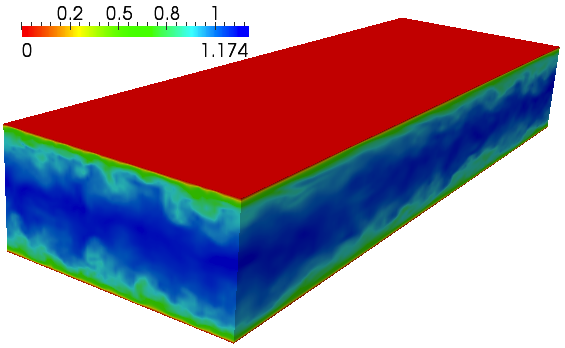
\includegraphics[width=12cm]{img/ChanCont.png}
\caption{Velocity profile of the turbulent channel flow (quasi-3D).}
\label{f:incns:turbchanflow}
\end{center}
\end{figure}


\subsection{Turbulent Pipe Flow}
In this example we simulate flow in a pipe at Reynolds number 3000 using a mixed
spectral/hp element and Fourier discretisation. The Fourier expansion is used in
the streamwise direction in this case and the spectral/hp elements are used to
capture the circular cross-section.

\subsubsection{Input File}
The circular pipe has diameter $D=1$, the 2D mesh is composed of 64
quadrilateral elements and the streamwise direction is discretised with 128
Fourier modes. An illustrative diagram of the discretisation is given in
Figure~\ref{f:incns:turbpipemesh}.

\begin{figure}
\begin{center}
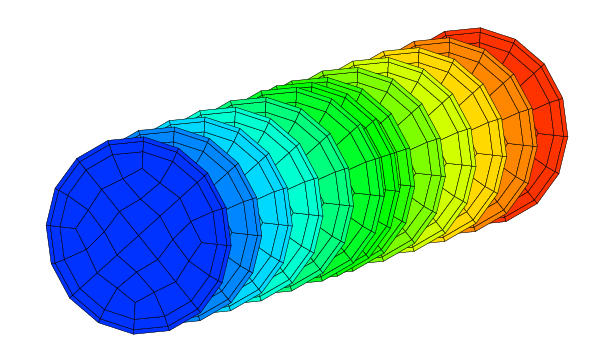
\includegraphics[width=10cm]{img/PipeDomain.png}
\caption{Domain for the turbulent pipe flow problem.}
\label{f:incns:turbpipemesh}
\end{center}
\end{figure}

The input file for this example is \inlsh{Pipe\_turb.xml}. We use 7th-order
lagrange polynomials through the Gauss-Lobatto-Legendre points for the
quadrilateral expansions.
\begin{lstlisting}[style=XMLStyle]
<E COMPOSITE="C[0]" NUMMODES="8" FIELDS="u,v,w,p" TYPE="GLL_LAGRANGE_SEM" />
\end{lstlisting}
We set the Fourier options, as in the previous example, except using 128
modes and a length of 5 non-dimensional units. A small amplitude noise is also
added to the initial condition, which is a plug profile, to help stimulate
transition. Since the streamwise direction is the Fourier direction, we must
necessarily use a body force to drive the flow.

\subsubsection{Running the solver}
In this example we will run the solver in parallel. Due to the large number of
Fourier modes and relatively few elements, it is more efficient to parallelise
in the streamwise direction. We can specify this by providing an additional flag
to the solver, \inlsh{--npz}. This indicates the number of partitions in the
z-coordinate. In this example, we will only run two processes. We therefore
would specify \inlsh{--npz 2} to ensure parallelisation only occurs in the
Fourier direction.

To improve the efficiency of the solver further, we would prefer to solve
the Helmholtz problems within the spectral/hp element planes using a
direct solver (since no parallelisation is necessary). The default when
running in parallel is to use an iterative solver, so we explicitly
specify the type of algorithm to use in the session file solver
information:
\begin{lstlisting}[style=XMLStyle]
<I PROPERTY="GlobalSysSoln" VALUE="DirectStaticCond" />
\end{lstlisting}

The solver can now be run as follows
\begin{lstlisting}[style=BashInputStyle]
mpirun -np 2 IncNavierStokesSolver --npz 2 Pipe_turb.xml
\end{lstlisting}

When the pipe transitions, the result should look similar to
Figure~\ref{f:incns:turbpipeflow}.

\begin{figure}
\begin{center}
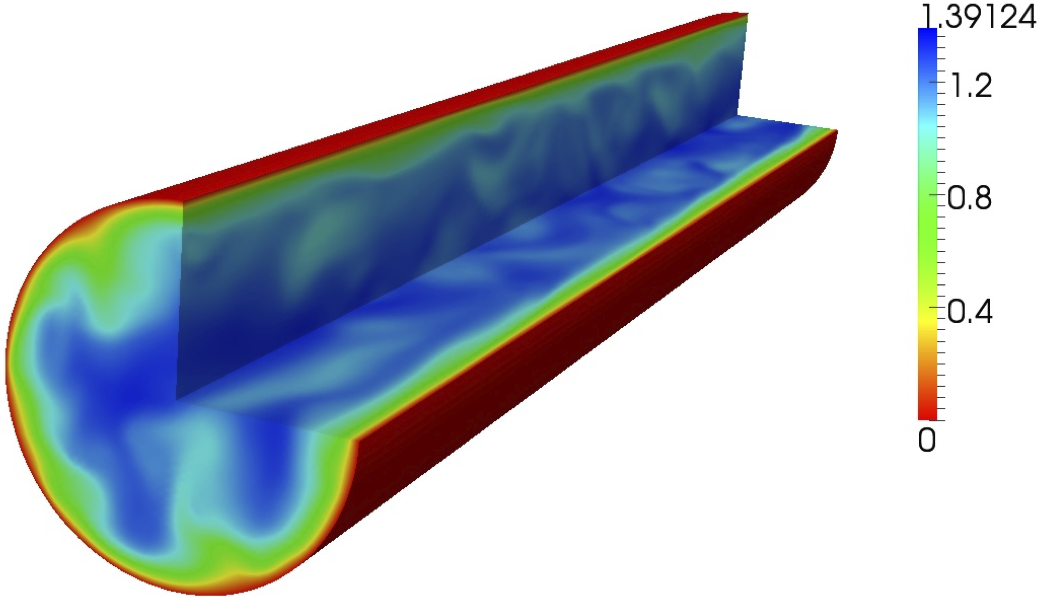
\includegraphics[width=12cm]{img/PipeCont.png}
\caption{Velocity profile of the turbulent pipe flow (quasi-3D).}
\label{f:incns:turbpipeflow}
\end{center}
\end{figure}



\subsection{Aortic Blood Flow}
The following example demonstrates the application of the
\hyperref[IncNSsolver]{incompressible Navier-Stokes solver} using the
\hyperref[VCSscheme]{Velocity Correction Scheme} algorithm for modelling viscid
Newtonian blood flow in a region of a rabbit descending thoracic aorta with
intercostal branch pairs. Such studies are necessary to understand the effect
local blood flow changes have on cardiovascular diseases such as
atherosclerosis.

In the following we will numerically solve for the three dimensional velocity
and pressure field for steady boundary conditions. The Reynolds number under
consideration is 300, which is physiologically relevant.

\textbf{Geometry}

The geometry under consideration is a segment of a rabbit descending aorta with two pairs of intercostal arteries branching off. The inlet has a diameter $D=3.32mm$.

\begin{figure}
\begin{center}
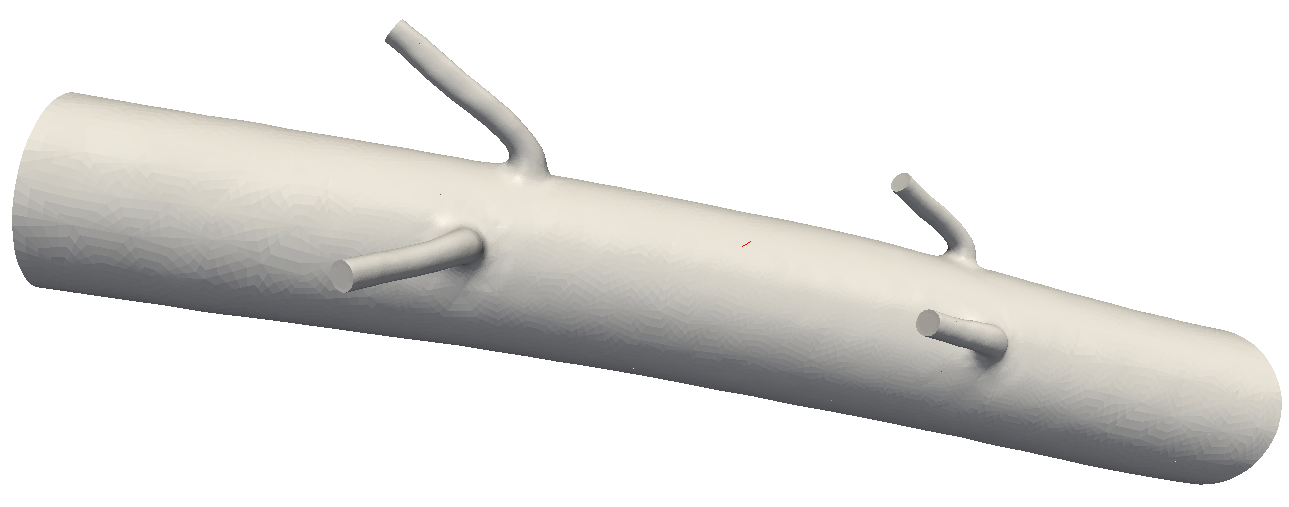
\includegraphics[width=10cm]{img/IntercostalGeometry.png}
\caption{Reduced region of rabbit descending thoracic aorta.}
\end{center}
\end{figure}

In order to capture the physics of the flow in the boundary layer, a thin layer consisting of prismatic elements is created adjacent to the surface, and curved using spherigons. The interior consist of tetrahedral elements.

\begin{figure}
\begin{center}
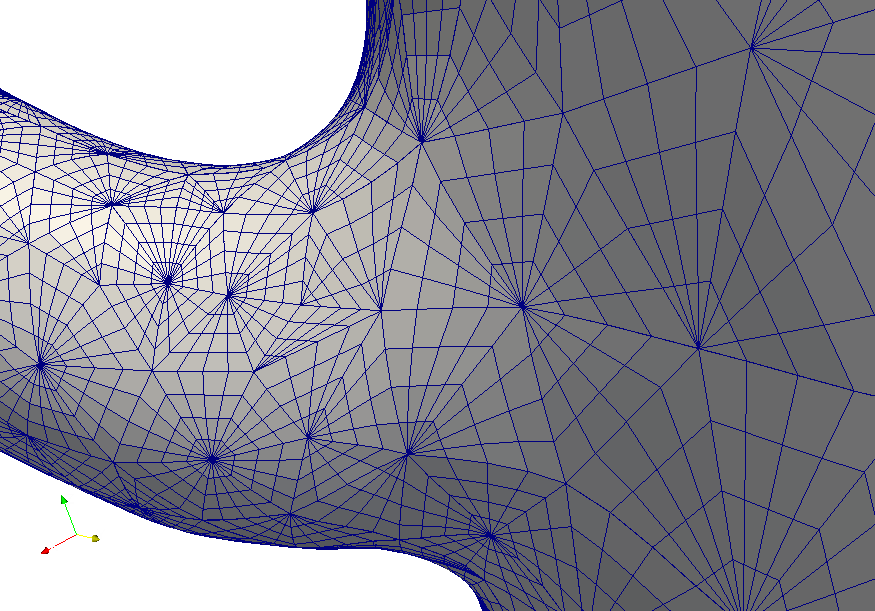
\includegraphics[width=7cm]{img/spherigons.png}
\caption{Surface mesh indicating curved surface elements at a branch location.}
\end{center}
\end{figure}


\textbf{Input parameters}

\subsubsection{Expansion:~} In this example we will use a fourth order polynomial expansion. There are two composites defined here since we have both prismatic and tetrahedral elements.
\begin{lstlisting}[style=XMLStyle]
<EXPANSIONS>
    <E COMPOSITE="C[0]" NUMMODES="5" TYPE="MODIFIED" FIELDS="u,v,w,p" />
    <E COMPOSITE="C[1]" NUMMODES="5" TYPE="MODIFIED" FIELDS="u,v,w,p" />
</EXPANSIONS>
\end{lstlisting}

\subsubsection{Solver information:~}
\begin{lstlisting}[style=XMLStyle]
<SOLVERINFO>
    <I PROPERTY="SolverType" VALUE="VelocityCorrectionScheme" />
    <I PROPERTY="EQTYPE" VALUE="UnsteadyNavierStokes" />
    <I PROPERTY="AdvectionForm" VALUE="Convective" />
    <I PROPERTY="Projection" VALUE="Galerkin" />
    <I PROPERTY="TimeIntegrationMethod" VALUE="IMEXOrder1" />
</SOLVERINFO>
\end{lstlisting}

\subsubsection{Parameters:~} Since we are prescribing a Reynolds number of 300, and to simplify the problem definition, we set the mean inlet velocity to 1, this allows us to define the kinematic viscosity as $\nu = \frac{UD}{Re}=\frac{3.32}{300} = 1/90.36$.

\begin{lstlisting}[style=XMLStyle]
<PARAMETERS>
    <P> TimeStep       = 0.0005     </P>
    <P> NumSteps       = 1600       </P>
    <P> IO_CheckSteps  = 200        </P>
    <P> IO_InfoSteps   = 50         </P>
    <P> Kinvis         = 1.0/90.36  </P>
</PARAMETERS>
\end{lstlisting}

\subsubsection{Boundary conditions:~} For the purpose of this example a blunted inlet velocity profile has been prescribed. Ideally to obtain more significant results, the velocity profile at the inlet would be obtained from previous simulations on the complete rabbit aorta (including aortic root, aortic arch, and descending aorta with all 5 pairs of intercostal arteries), where a blunted profile at the aortic root is a better representation of reality.

Dirichlet boundary conditions are imposed for the velocity at the inlet, as well as on the wall to account for the no-slip condition. Neumann boundary conditions are imposed for the velocity field at the outlets where fully developed flow is imposed.

\begin{lstlisting}[style=XMLStyle]
<BOUNDARYREGIONS>
    <B ID="0"> C[2] </B>          <!-- Inlet -->
    <B ID="1"> C[3,4,5,6] </B>    <!-- intercostal outlets -->
    <B ID="2"> C[7] </B>          <!-- outlet -->
    <B ID="3"> C[8] </B>          <!-- wall -->
</BOUNDARYREGIONS>

<BOUNDARYCONDITIONS>
    <REGION REF="0">
        <D VAR="u" VALUE="0.024" />
        <D VAR="v" VALUE="-0.064" />
        <D VAR="w" VALUE="-0.998" />
        <N VAR="p" USERDEFINEDTYPE="H" VALUE="0" />
    </REGION>
    <REGION REF="1">
        <N VAR="u" VALUE="0" />
        <N VAR="v" VALUE="0" />
        <N VAR="w" VALUE="0" />
        <D VAR="p" VALUE="0" />
    </REGION>
    <REGION REF="2">
        <N VAR="u" VALUE="0" />
        <N VAR="v" VALUE="0" />
        <N VAR="w" VALUE="0" />
        <D VAR="p" VALUE="0" />
    </REGION>
    <REGION REF="3">
        <D VAR="u" VALUE="0" />
        <D VAR="v" VALUE="0" />
        <D VAR="w" VALUE="0" />
        <N VAR="p" USERDEFINEDTYPE="H" VALUE="0" />
    </REGION>
</BOUNDARYCONDITIONS>
\end{lstlisting}

\subsubsection{Functions:~}
\begin{lstlisting}[style=XMLStyle]
<FUNCTION NAME="InitialConditions">
    <E VAR="u" VALUE="0" />
    <E VAR="v" VALUE="0" />
    <E VAR="w" VALUE="0" />
    <E VAR="p" VALUE="0" />
</FUNCTION>
\end{lstlisting}

\subsubsection{Results}
We can visualise the internal velocity field by applying a volume render filter in ParaView.

\begin{figure}
\begin{center}
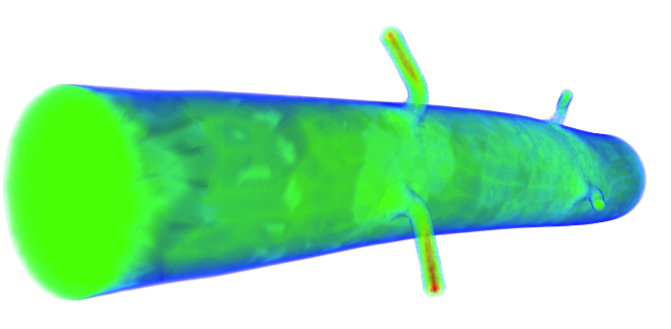
\includegraphics[width=10cm]{img/velocityRendered.png}
\caption{The solved-for velocity field.}
\end{center}
\end{figure}

It is possible to visualise the wall shear stress distribution by running the FldAddWSS utility.

\begin{figure}
\begin{center}
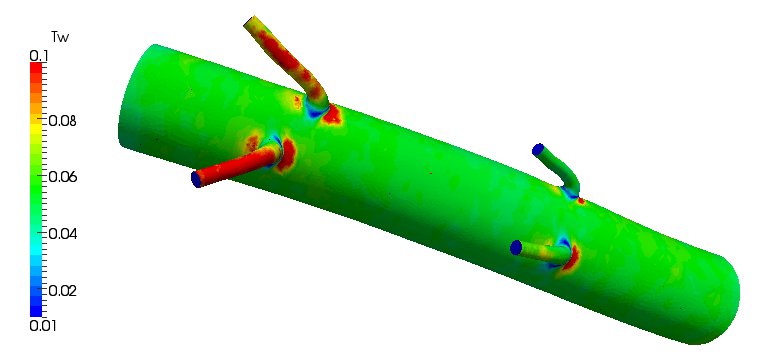
\includegraphics[width=12cm]{img/WSS.png}
\caption{Non-dimensional wall shear stress distribution.}
\end{center}
\end{figure}

\subsection{finite-strip modeling of flow past flexible cables}

As a computationally efficient model, strip theory-based modeling technique has been proposed previously to predict vortex-induced vibration (VIV) for higher Reynolds number flows. In the strip theory-based model, the fluid flow solution is obtained on a series of 2D computational planes (also called as “strips”) along the riser’s axis direction. These strips then are coupled with each other through structural dynamic model of the riser, and then VIV response prediction is achieved by the strip-structure interactions.In the 2D strip theory, it is assumed that the flow is purely two-dimensional without spanwise correlation, which allows the problems to be split into various 2D planes. A consequence of 2D strip solution under this assumption is that it is unable to reflect the influence of spanwise wake turbulence on the structural dynamics. In order to overcome this shortcoming, we proposed a new module in the framework of Nektar++, in which a spanwise scale is locally allocated to each one of the strips, so that the spanwise velocity correlation is reconstructed in the flow field within each strips. In particular, this model lets the fluid domain to be divided in $N$ strips with thickness ratio of $L_{z}/D$ and evenly distributed along the spanwise ($z$) direction. The gap between the neighboring strips, represented by $L_{g}$, satisfies relation $L_{c}=N(L_{z}+L_{g})$. Since the strip in this model has finite scale in the $z$-direction, we named it as finite strip to distinguish from traditional 2D strip plane. Next, the flow dynamics within each individual strips are modeled by viscous incompressible Navier-Stokes equations, while a tensioned beam model is employed to govern the dynamics of the flexible structures. In this example, we will show how to perform a finite-strip model to predict the vortex-induced vibration responses of flexible cables. Let us consider a vortex-induced vibration of a slender cable with an aspect ratio of $L_z/D$=4$\pi$, which is immersed in uniform flows at Re=100.

\subsubsection{Input File}

The cable with a mass ratio (defined as the ratio of the total oscillating mass to the mass of displaced fluid) of 1 has diameter $D=1$, the 2D mesh is composed of 284 quadrilateral elements. The spanwise direction is split in 16 strips with thickness ratio of $L_c/D$=$\pi$/8 and one pair of complex Fourier modes for each one of the strips. We will use a sixth order polynomial expansion for the spectral element and the input file for this example is \inlsh{CylFlow\_HomoStrip.xml}.



\begin{lstlisting}[style=XMLStyle]
<E COMPOSITE="C[73]" NUMMODES="6" TYPE="MODIFIED" FIELDS="u,v,w,p" />
\end{lstlisting}

To use the finite strip routines we need just to insert a flag of \inlsh{"HomoStrip"} in the solver information as below, in addition, we need to specify the types of vibration and support ends for the cables. In this case, the vibration type is specified as \inlsh{VALUE="CONSTRAINED"}, which means that the cable's vibration is constrained only in the crossflow direction. Other options include \inlsh{VALUE="FREE"} and \inlsh{"FORCED"}, respectively corresponding to the free vibrations in both streamwise and crossflow directions and forced vibration by specified functions given in input file. For the support ends of the cable, another option of \inlsh{VALUE="PINNED-PINNED"} is available for the simulations, which satisfies the condition of zero values of displacements on the support ends.

\subsubsection{Solver information:~}
\begin{lstlisting}[style=XMLStyle]
        <SOLVERINFO>
            <I PROPERTY="HomoStrip" VALUE="True"/>
            <I PROPERTY="VibrationType" VALUE="CONSTRAINED"/>
            <I PROPERTY="SupportType" VALUE="FREE-FREE"/>
        </SOLVERINFO>
\end{lstlisting}
        
\subsubsection{Parameters}

All the simulation parameters are specified in the section as follows.

    \begin{lstlisting}[style=XMLStyle]
        <PARAMETERS>
            <P> LZ            = PI/8             </P> <!--thickness ratio-->
            <P> LC            = 4*PI             </P> <!--aspect ratio-->
            <P> A             = 0.025            </P>
            <P> omega         = 1.0              </P>
            <P> PROC_Z        = 16               </P>
            <P> Strip_Z       = 16               </P> <!--number of the strips-->
            <P> DistStrip     = PI/4             </P> <!--distance of the strips-->
            <P> StructStiff   = 0.02             </P>  
            <P> StructRho     = 2.0              </P>
            <P> CableTension  = 8.82             </P>
            <P> BendingStiff  = 0.0              </P>
            <P> FictDamp      = 0.0              </P>
            <P> FictMass      = 3.0              </P>
        </PARAMETERS>
     \end{lstlisting}    

\subsubsection{Running the solver}
In this example we will run the solver in parallel. We can specify the number of the strips by providing an additional flag to the solver, –nsz. In this example, we will run 16 strips, therefore it would be specified as –nsz 16. The solver can now be run as follows    

\begin{lstlisting}[style=BashInputStyle]
mpirun -np 16 IncNavierStokesSolver  CylFlow_HomoStrip.xml --npz 16 --nsz 16
\end{lstlisting}

The simulation results are illustrated in spanwise vorticity contours in Figure \ref{f:incns:finite-strip-modeling}. The wake response of the cable appears as standing wave patter in the earlier stage and then it transitions into traveling wave response, as shown in this figure.  

\begin{figure}
\begin{center}
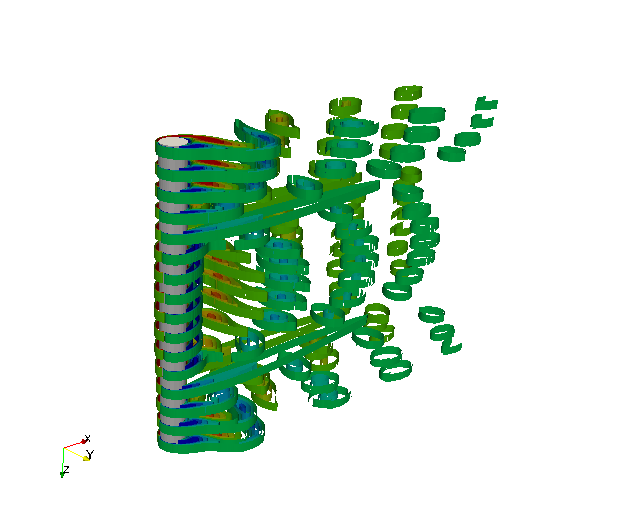
\includegraphics[width=7cm]{img/strip-16-time-100.png}
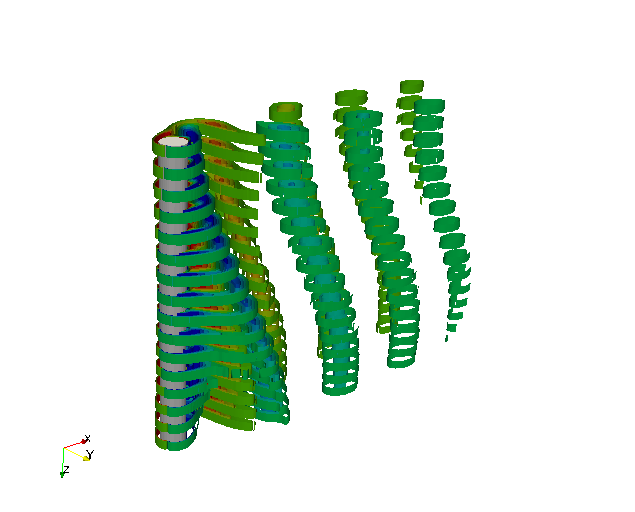
\includegraphics[width=7cm]{img/strip-16-time-600.png}
\caption{Spanwise vorticity contours in standing wave and traveling wave patterns predicted in finite strip modeling.}
\label{f:incns:finite-strip-modeling}
\end{center}
\end{figure}

 \subsection{2D direct stability analysis of the channel flow}

  In this example, it will be illustrated how to perform a direct stability analysis using Nektar++. Let us consider a canonical stability problem, the flow in a channel which is confined in the wall-normal direction between two infinite plates (Poiseuille flow) at Reynolds number 7500. This problem is a particular case of the stability solver for the IncNavierStokesSolver.

 \subsubsection{Background}

  We consider the linearised Incompressible Navier-Stokes equations:

  \begin{subequations}
  \begin{equation}
    \frac{\partial \mathbf{u'}}{\partial t} + \mathbf{U} \cdot  \nabla \mathbf{u'}+\mathbf{u'} \cdot \nabla \mathbf{U} = -\nabla p + \nu \nabla^2 \mathbf{u'} + \mathbf{f}
  \end{equation}

  \begin{equation}
  \nabla \cdot \mathbf{u'} = 0
  \end{equation}
  \end{subequations}

  We are interested to compute the leading eigenvalue of the system using the Arnoldi method.

  \subsubsection{Geometry}

   The geometry under consideration is a 2D channel.

   \subsubsection{Mesh Definition}

   In the \texttt{GEOMETRY} section, the dimensions of the problem are defined. Then, the coordinates (\texttt{XSCALE}, \texttt{YSCALE}, \texttt{ZSCALE}) of each vertices of each element are specified. As this input file defines a two-dimensional problem: \texttt{ZSCALE = 0}.

  \begin{lstlisting}[style=XMLStyle]
<GEOMETRY DIM="2" SPACE="2">
        <VERTEX>
            <V ID="0">3.142e+00 1.000e+00 0.000e+00</V>
            ...
            <V ID="62">-3.142e+00 -1.000e+00 0.000e+00</V>
        </VERTEX>
\end{lstlisting}

Edges can now be defined by two vertices.

  \begin{lstlisting}[style=XMLStyle]
<EDGE>
            <E ID="0">    0  1   </E>
            ...
            <E ID="109">   62  55   </E>
        </EDGE>
\end{lstlisting}


In the \texttt{ELEMENT} section, the tag \texttt{T} and \texttt{Q} define respectively triangular and quadrilateral element. Triangular elements are defined by a sequence of three edges and quadrilateral elements by a sequence of four edges.

  \begin{lstlisting}[style=XMLStyle]
        <ELEMENT>
            <Q ID="0">    0     1     2     3 </Q>
            ...
            <Q ID="47">  107   108   109    95 </Q>
        </ELEMENT>
        \end{lstlisting}

Finally, collections of elements are listed in the \texttt{COMPOSITE} section and the \texttt{DOMAIN} section specifies that the mesh is composed by all the triangular and quadrilateral elements. The other composites will be used to enforce boundary conditions.

  \begin{lstlisting}[style=XMLStyle]
              <COMPOSITE>
            <C ID="0"> Q[0-47] </C>
            <C ID="1"> E[17,31,44,57,70,83,96,109,0,19,32,45,58,71,84,97] </C> //wall
            <C ID="2"> E[3,6,9,12,15,18] </C>//inflow
            <C ID="3"> E[98,100,102,104,106,108] </C> //outflow
        </COMPOSITE>
        <DOMAIN> C[0] </DOMAIN>
</GEOMETRY>
  \end{lstlisting}

  \subsubsection{Expansion}

  This section defines the polynomial expansions used on each composites. For this example we will use a 10th order polynomial, i.e. $P=11$.

  \begin{lstlisting}[style=XMLStyle]
<EXPANSIONS>
     <E COMPOSITE="C[0]" NUMMODES="11" FIELDS="u,v,p" TYPE="MODIFIED" />
</EXPANSIONS>
  \end{lstlisting}

  \subsubsection{Solver Info}

  In this example the \texttt{EvolutionOperator} must be \texttt{Direct} to consider the linearised Navier-Stokes equations and the \texttt{Driver} was set up to \texttt{ModifiedArnoldi} for the solution of the eigenproblem.

    \begin{lstlisting}[style=XMLStyle]
      <SOLVERINFO>
      <I PROPERTY="SolverType"        VALUE="VelocityCorrectionScheme"/>
      <I PROPERTY="EQTYPE"            VALUE="UnsteadyNavierStokes"/>
      <I PROPERTY="EvolutionOperator" VALUE="Direct"/>
      <I PROPERTY="Projection"        VALUE="Galerkin"/>
      <I PROPERTY="Driver"            VALUE= "ModifiedArnoldi" />
      <I PROPERTY="TimeIntegrationMethod" VALUE="IMEXOrder1" />
    </SOLVERINFO>
      \end{lstlisting}


\subsubsection{Parameters}

All the stability parameters are specified in this section.

    \begin{lstlisting}[style=XMLStyle]
<PARAMETERS>
      <P> TimeStep      = 0.002 </P>
      <P> NumSteps      = 500 </P>
      <P> IO_CheckSteps = 1000    </P>
      <P> IO_InfoSteps  = 10    </P>
      <P> Re            = 7500     </P>
      <P> Kinvis         =1./Re   </P>
      <P> kdim           =16   </P>
      <P> nvec           =2   </P>
      <P> evtol          =1e-5</P>
      <P> nits           =5000 </P>
   </PARAMETERS>
         \end{lstlisting}


\subsubsection{Boundary Conditions}

    \begin{lstlisting}[style=XMLStyle]
 <BOUNDARYREGIONS>
            <B ID="0"> C[1] </B>
            <B ID="1"> C[2] </B>
            <B ID="2"> C[3] </B>
        </BOUNDARYREGIONS>

        <BOUNDARYCONDITIONS>
            <REGION REF="0">
                <D VAR="u" VALUE="0" />
                <D VAR="v" VALUE="0" />
                <N VAR="p" USERDEFINEDTYPE="H" VALUE="0" />
            </REGION>
            <REGION REF="1">
                <P VAR="u" VALUE="[2]" />
                <P VAR="v" VALUE="[2]" />
                <P VAR="p" VALUE="[2]" />
            </REGION>
            <REGION REF="2">
                <P VAR="u" VALUE="[1]" />
                <P VAR="v" VALUE="[1]" />
                <P VAR="p" VALUE="[1]" />
            </REGION>
        </BOUNDARYCONDITIONS>
                 \end{lstlisting}

\subsubsection{Function}

We need to set up the base flow that can be specified as a function \texttt{BaseFlow}. In case the base flow is not analytical, it can be generated by means of the \texttt{Nonlinear} evolution operator using the same mesh and polynomial expansion. The initial guess is specified in the \texttt{InitialConditions} functions and can be both analytical or a file. In this example it is read from a file.

    \begin{lstlisting}[style=XMLStyle]
<FUNCTION NAME="BaseFlow">
            <F VAR="u,v,p" FILE="ChanStability.bse" />
        </FUNCTION>

        <FUNCTION NAME="InitialConditions">
            <F VAR="u,v,p" FILE="ChanStability.rst" />
        </FUNCTION>
                         \end{lstlisting}



\subsubsection{Usage}

\texttt{IncNavierStokesSolver ChanStability.xml}


\subsubsection{Results}

The stability simulation takes about 250 iterations to converge and the dominant eigenvalues (together with the respective eigenvectors) will be printed. In this case it was found $    \lambda_{1,2}=1.000224 \times e^{\pm 0.24984i}$. Therefore, since the magnitude of the eigenvalue is larger than 1, the flow is absolutely unstable. It is possible to visualise the eigenvectors using the post-processing utilities. The figure shows the profile of the two eigenmode component, which shows the typical Tollmien - Schlichting waves that arise in viscous boundary layers.

\begin{figure}[!htbp]
\centering
 {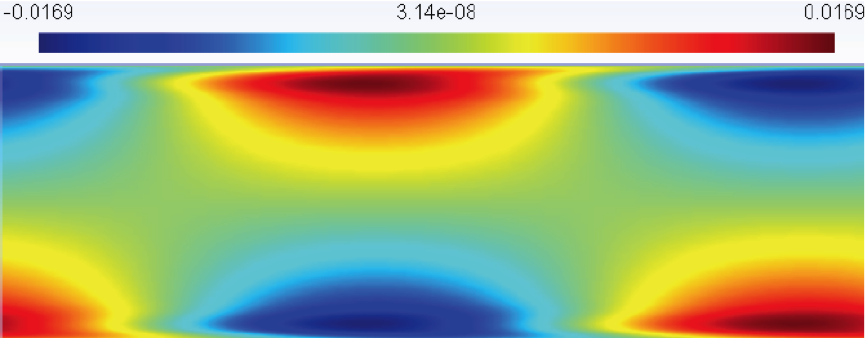
\includegraphics[width=1 \textwidth]{img/chan_u.png}}
   \caption {}
\end{figure}

\begin{figure}[!htbp]
\centering
 {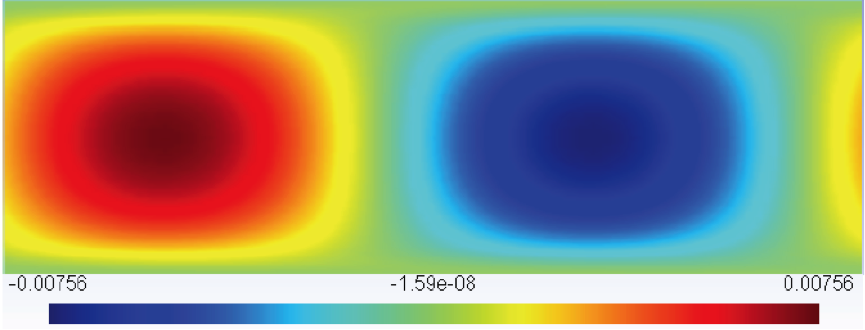
\includegraphics[width=1 \textwidth]{img/chan_v}}
    \caption {}
\end{figure}

 \subsection{2D adjoint stability analysis of the channel flow}

 In this example, it will be illustrated how to perform an adjoint stability analysis using Nektar++. Let us consider a canonical stability problem, the flow in a channel which is confined in the wall-normal direction between two infinite plates (Poiseuille flow) at Reynolds number 7500

 \subsubsection{Background}

  We consider the equations:

  \begin{subequations}
  \begin{equation}
  -\frac{\partial \mathbf{u}^*}{\partial t}+(\mathbf{U} \cdot \nabla)\mathbf{u}^*+(\nabla \mathbf{U})^T \cdot \mathbf{u}^*=-\nabla p^*+\frac{1}{Re} \nabla^2 \mathbf{u}
  \end{equation}

  \begin{equation}
  \nabla \cdot \mathbf{u}^*=0
  \end{equation}
  \end{subequations}

  We are interested in computing the leading eigenvalue of the system using the Arnoldi method.

 \subsubsection{Geometry \& Mesh}

 The geometry and mesh are the same ones used for the direct stability analysis in the previous example.

 \subsubsection{Solver Info}

 This sections defines the problem solved. In this example the \texttt{EvolutionOperator} must be \texttt{Adjoint} to consider the adjoint Navier-Stokes equations and the \texttt{Driver} was set up to \texttt{ModifiedArnoldi} for the solution of the eigenproblem.

    \begin{lstlisting}[style=XMLStyle]
<SOLVERINFO>
      <I PROPERTY="SolverType"        VALUE="VelocityCorrectionScheme"/>
      <I PROPERTY="EQTYPE"            VALUE="UnsteadyNavierStokes"/>
      <I PROPERTY="EvolutionOperator" VALUE="Adjoint"/>
      <I PROPERTY="Projection"        VALUE="Galerkin"/>
      <I PROPERTY="Driver"            VALUE= "ModifiedArnoldi" />
      <I PROPERTY="TimeIntegrationMethod" VALUE="IMEXOrder1" />
</SOLVERINFO>
  \end{subequations}

\textbf{Parameters}

    \begin{lstlisting}[style=XMLStyle]
<PARAMETERS>
      <P> TimeStep      = 0.002 </P>
      <P> NumSteps      = 500 </P>
      <P> IO_CheckSteps = 1000    </P>
      <P> IO_InfoSteps  = 10    </P>
      <P> Re            = 7500     </P>
      <P> Kinvis         =1./Re   </P>
      <P> kdim           =16   </P>
      <P> nvec           =2   </P>
      <P> evtol          =1e-5</P>
      <P> nits           =5000 </P>
</PARAMETERS>
  \end{lstlisting}

\subsubsection{Boundary Conditions}

    \begin{lstlisting}[style=XMLStyle]
 <BOUNDARYREGIONS>
            <B ID="0"> C[1] </B>
            <B ID="1"> C[2] </B>
            <B ID="2"> C[3] </B>
        </BOUNDARYREGIONS>

        <BOUNDARYCONDITIONS>
            <REGION REF="0">
                <D VAR="u" VALUE="0" />
                <D VAR="v" VALUE="0" />
                <N VAR="p" USERDEFINEDTYPE="H" VALUE="0" />
            </REGION>
            <REGION REF="1">
                <P VAR="u" VALUE="[2]" />
                <P VAR="v" VALUE="[2]" />
                <P VAR="p" VALUE="[2]" />
            </REGION>
            <REGION REF="2">
                <P VAR="u" VALUE="[1]" />
                <P VAR="v" VALUE="[1]" />
                <P VAR="p" VALUE="[1]" />
            </REGION>
        </BOUNDARYCONDITIONS>
  \end{lstlisting}


\subsubsection{Functions}

We need to set up the base flow that can be specified as a function \texttt{BaseFlow}. In case the base flow is not analytical, it can be generated by means of the \texttt{Nonlinear} evolution operator using the same mesh and polynomial expansion.

    \begin{lstlisting}[style=XMLStyle]
        <FUNCTION NAME="BaseFlow">
            <F VAR="u,v,p" FILE="ChanStability.bse" />
        </FUNCTION>
  \end{lstlisting}

  The initial guess is specified in the \texttt{InitialConditions} functions and can be both analytical or a file. In this example it is read from a file.

      \begin{lstlisting}[style=XMLStyle]
        <FUNCTION NAME="InitialConditions">
            <F VAR="u,v,p" FILE="ChanStability.rst" />
        </FUNCTION>
          \end{lstlisting}

\subsubsection{Usage}

\texttt{IncNavierStokesSolver ChanStability\_adj.xml}

\subsubsection{Results}

The equations will then be evolved backwards in time (consistently with the negative sign in front of the time derivative) and the leading eigenvalues will be computed after about 300 iterations. It is interesting to note that their value is the same one computed for the direct problem, but the eigenmodes present a different shape.


\begin{figure}[!htbp]
\centering
 {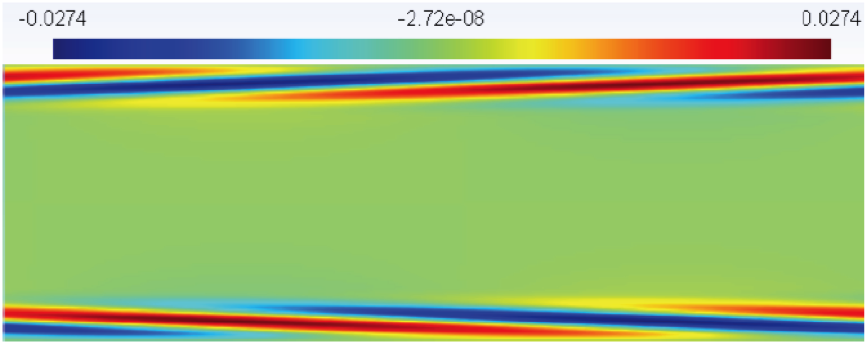
\includegraphics[width=1 \textwidth]{img/chan_u_adj.png}}
   \caption {}
\end{figure}

\begin{figure}[!htbp]
\centering
 {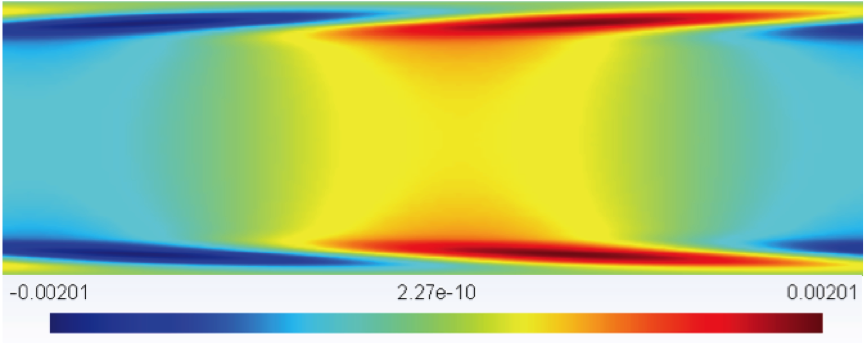
\includegraphics[width=1 \textwidth]{img/chan_v_adj}}
    \caption {}
\end{figure}

\subsection{2D Transient Growth analysis of a flow past a backward-facing step}

In this section it will be described how to perform a transient growth stability analysis using Nektar++. Let us consider a flow past a backward-facing step (figure \ref{bfs_geo}). This is an important case because it allows us to understand  the effects of separation caused by abrupt changes in the geometry and it is a common geometry in several studies of flow control and turbulence of separated flow.

\begin{figure}[!htbp]
\centering
 {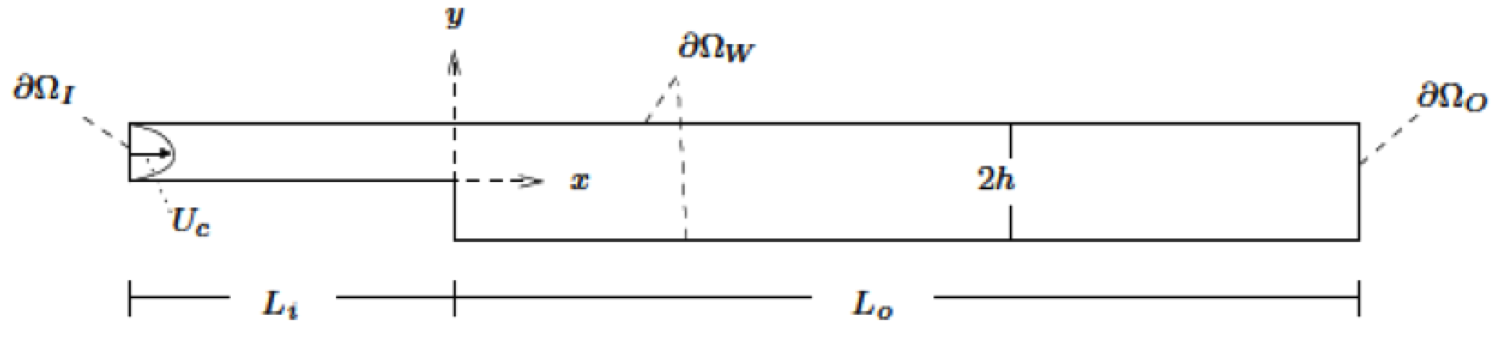
\includegraphics[width=1 \textwidth]{img/bfs_geo}}
    \caption {}\label{bfs_geo}
\end{figure}

\subsubsection{Background}

Transient growth analysis allows us to study the presence of convective instabilities that can arise in stable flows. Despite the fact that these instabilities will decay for a long time (due to the stability of the flow), they can produce significant increases in the energy of perturbations. The phenomenon of transient growth is associated with the non-normality of the linearised Navier-Stokes equations and it consists in computing the perturbation that leads to the highest energy growth for a fixed time horizon.

\subsubsection{Input Parameters}

In the \texttt{GEOMETRY} section, the dimensions of the problem are defined. Then, the coordinates (\texttt{XSCALE}, \texttt{YSCALE}, \texttt{ZSCALE}) of each vertices are specified. As this input file defines a two-dimensional problem: \texttt{ZSCALE = 0}.

      \begin{lstlisting}[style=XMLStyle]
<GEOMETRY DIM="2" SPACE="2">
   <VERTEX>
       <V ID="0">3.000e+00 -1.000e+00 0.000e+00</V>
       ...
       <V ID="399">-1.000e+01 0.000e+00 0.000e+00</V>
   </VERTEX>
     \end{lstlisting}

Edges can now be defined by two vertices.

      \begin{lstlisting}[style=XMLStyle]
<EDGE>
       <E ID="0">    0  1   </E>
       ...
       <E ID="828">  399  394   </E>
   </EDGE>
        \end{lstlisting}

In the \texttt{ELEMENT} section, the tag \texttt{T} and \texttt{Q} define respectively triangular and quadrilateral element. Triangular elements are defined by a sequence of three edges and quadrilateral elements by a sequence of four edges.

      \begin{lstlisting}[style=XMLStyle]
<ELEMENT>
       <T ID="0">    0     1     2 </T>
       ...
       <T ID="209">  333   314   332 </T>
       <Q ID="210">  334   335   336     0 </Q>
       ...
       <Q ID="429">  826   827   828   818 </Q>
   </ELEMENT>
        \end{lstlisting}

Finally, collections of elements are listed in the \texttt{COMPOSITE} section and the \texttt{DOMAIN} section specifies that the mesh is composed by all the triangular and quadrilateral elements. The other composites will be used to enforce boundary conditions.

      \begin{lstlisting}[style=XMLStyle]
<COMPOSITE>
       <C ID="0"> T[0-209] </C>
       <C ID="1"> Q[210-429] </C>
       <C ID="2"> E[2-3,7,10,16,21,2,...,828] </C>
       <C ID="3"> E[821,823,825,827] </C>
       <C ID="4"> E[722,724,726,728] </C>
   </COMPOSITE>

   <DOMAIN> C[0,1] </DOMAIN>
</GEOMETRY>
        \end{lstlisting}

\subsubsection{Expansion}

For this example we will use a 6th order polynomial, i.e. $P=7$:

      \begin{lstlisting}[style=XMLStyle]
<EXPANSIONS>
    <E COMPOSITE="C[0]" NUMMODES="7" FIELDS="u,v,p" TYPE="MODIFIED" />
    <E COMPOSITE="C[1]" NUMMODES="7" FIELDS="u,v,p" TYPE="MODIFIED" />
</EXPANSIONS>
        \end{lstlisting}

\subsubsection{Solver Information}

This sections defines the problem solved. In this example the \texttt{EvolutionOperator} must be \texttt{TransientGrowth} and the \texttt{Driver} was set up to \texttt{Arpack} for the solution of the eigenproblem.

      \begin{lstlisting}[style=XMLStyle]
 <SOLVERINFO>
            <I PROPERTY="EQTYPE"                VALUE="UnsteadyNavierStokes"    />
            <I PROPERTY="EvolutionOperator"     VALUE="TransientGrowth"         />
            <I PROPERTY="Projection"            VALUE="Galerkin"                />
            <I PROPERTY="TimeIntegrationMethod" VALUE="IMEXOrder2"              />
            <I PROPERTY="SOLVERTYPE"            VALUE="VelocityCorrectionScheme"/>
            <I PROPERTY="Driver"                VALUE="Arpack"                  />
            <I PROPERTY="ArpackProblemType"     VALUE="LargestMag"              />
        </SOLVERINFO>
                \end{lstlisting}


\subsubsection{Parameters}

      \begin{lstlisting}[style=XMLStyle]
<PARAMETERS>
            <P> FinalTime       = 0.1                   </P>
            <P> TimeStep        = 0.005                 </P>
            <P> NumSteps        = FinalTime/TimeStep    </P>
            <P> IO_CheckSteps   = 1/TimeStep            </P>
            <P> IO_InfoSteps    = 1                     </P>
            <P> Re              = 500                   </P>
            <P> Kinvis          = 1.0/Re                </P>
            <P> kdim            = 4                     </P>
            <P> nvec            = 1                     </P>
            <P> evtol           = 1e-4                  </P>
        </PARAMETERS>
                        \end{lstlisting}


\subsubsection{Boundary Conditions}

      \begin{lstlisting}[style=XMLStyle]
 <BOUNDARYREGIONS>
            <B ID="0"> C[2] </B>    <!-- Wall -->
            <B ID="1"> C[3] </B>    <!-- Inlet -->
            <B ID="2"> C[4] </B>    <!-- Outlet -->
        </BOUNDARYREGIONS>

        <BOUNDARYCONDITIONS>
            <REGION REF="0">
                <D VAR="u" VALUE="0" />
                <D VAR="v" VALUE="0" />
                <N VAR="p" USERDEFINEDTYPE="H" VALUE="0" />
            </REGION>
            <REGION REF="1">
                <D VAR="u" VALUE="0" />
                <D VAR="v" VALUE="0" />
                <N VAR="p" USERDEFINEDTYPE="H" VALUE="0" />
            </REGION>
            <REGION REF="2">
                <D VAR="u" VALUE="0" />
                <D VAR="v" VALUE="0" />
                <N VAR="p" USERDEFINEDTYPE="H" VALUE="0" />
            </REGION>
        </BOUNDARYCONDITIONS>
                                \end{lstlisting}

\subsubsection{Functions}

We need to set up the base flow that can be specified as a function \texttt{BaseFlow}. In case the base flow is not analytical, it can be generated by means of the \texttt{Nonlinear} evolution operator using the same mesh and polynomial expansion.

      \begin{lstlisting}[style=XMLStyle]
<FUNCTION NAME="BaseFlow">
            <F VAR="u,v,p" FILE="bfs_tg-AR.bse" />
        </FUNCTION>
                                        \end{lstlisting}


The initial guess is specified in the \texttt{InitialConditions} functions and in this case is read from a file.

 \begin{lstlisting}[style=XMLStyle]
<FUNCTION NAME="InitialConditions">
            <F VAR="u,v,p" FILE="bfs_tg-AR.rst" />
        </FUNCTION>
                                        \end{lstlisting}


\subsubsection{Usage}

\texttt{IncNavierStokesSolver bfs\_tg-AR.xml}

\subsubsection{Results}

The solution will be evolved forward in time using the operator $\mathcal{A}$, then backward in time through the adjoint operator $\mathcal{A}^*$. The leading eigenvalue is $\lambda= 3.236204)$. This corresponds to the largest possible transient growth at the time horizon $\tau= 1$. The leading eigenmode is shown below. This is the optimal initial condition which will lead to the greatest growth when evolved under the linearised Navier-Stokes equations.


\begin{figure}[!htbp]
\centering
 {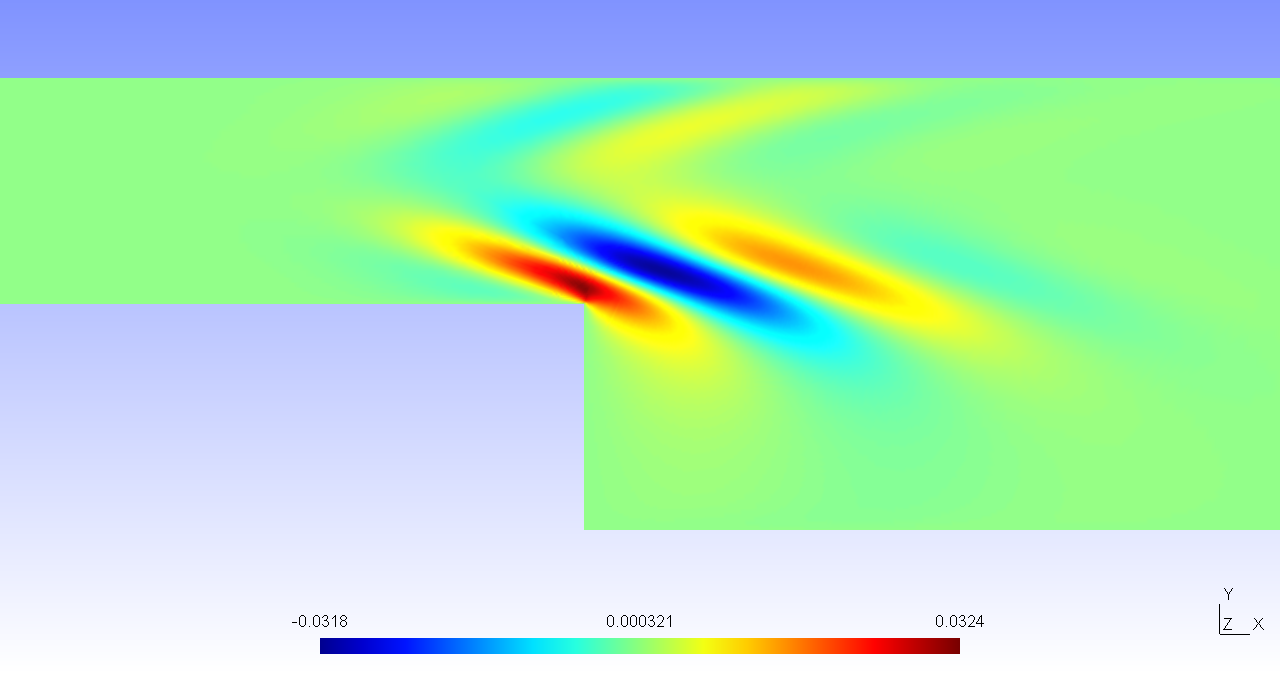
\includegraphics[width=1 \textwidth]{img/bfs_eig_u}}
   \caption {}
\end{figure}

\begin{figure}[!htbp]
\centering
 {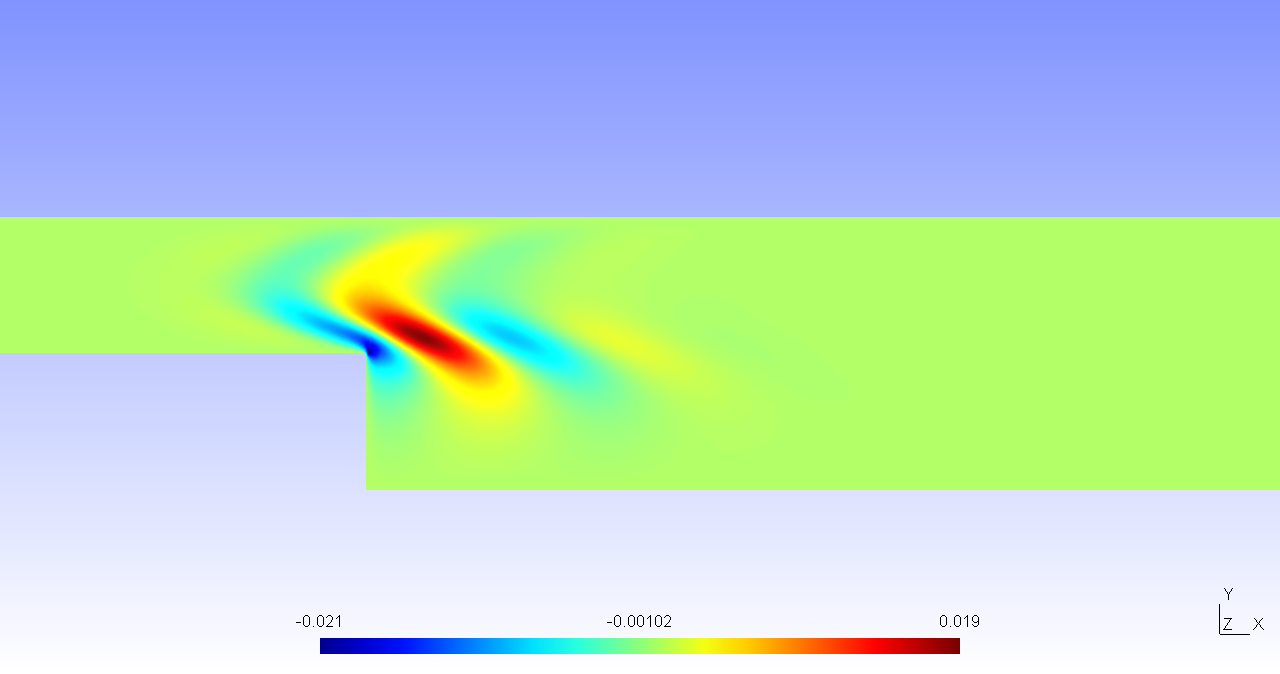
\includegraphics[width=1 \textwidth]{img/bfs_eig_v}}
    \caption {}
\end{figure}

It is possible to visualise the transient growth plotting the energy evolution over time if the system is initially perturbed with the leading eigenvector. This analysis was performed  for a time horizon $\tau= 60$. It can be seen that the energy grows in time reaching its maximum value at x = 24 and then decays, almost disappearing after 100 temporal units.


\begin{figure}[!htbp]
\centering
 {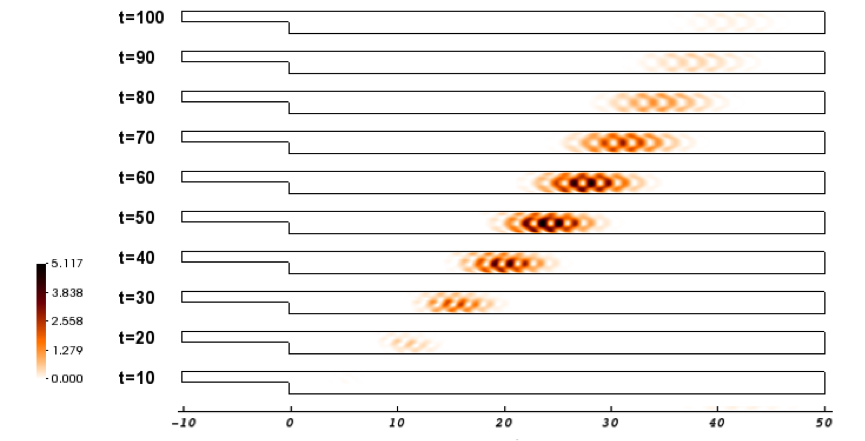
\includegraphics[width=1 \textwidth]{img/energy_bfs}}
   \caption {}
\end{figure}

\subsection{BiGlobal Floquet analysis of a of flow past a cylinder}

 In this example it will be described how to run a BiGlobal stability analysis for a time-periodic base flow using Nektar++. Let us consider a flow past a circular cylinder at $Re=220$ has a 2D time-periodic wake that is unstable to a 3D synchronous "mode A" instability.

 \begin{figure}[!htbp]
\centering
 {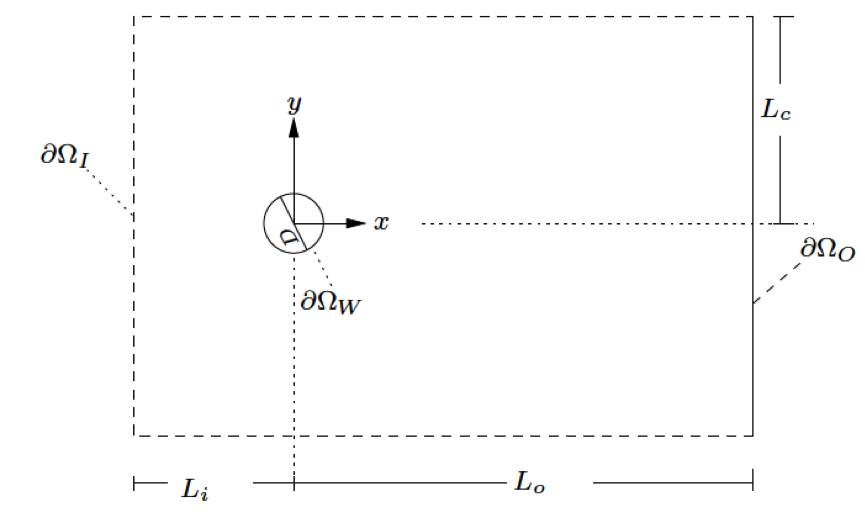
\includegraphics[width=1 \textwidth]{img/cylinder_geo}}
   \caption {}
\end{figure}


\subsubsection{Background}

The numerical solution of the fully three- dimensional linear eigenvalue problem is often computationally demanding and may not have significant advantages over performing a direct numerical simulation. Therefore, some simplifications are required; the most radical consist in considering that the base flow depends only on one spatial coordinate, assuming that the other two spatial coordinates are homogenous.  While this method offers a good prediction for the instability of boundary layers, it is not able to predict the instability of Hagen-Poiseuille flow in a pipe at all Reynolds numbers.  Between a flow that depends upon one and three-spatial directions, it is possible to consider a steady or time-periodic base flow depending upon two spatial directions and impose three-dimensional disturbances that are periodic in the the third homogeneous  spatial direction. This approach is known as BiGlobal stability analysis and it represents the extension of the classic linear stability theory; let us consider a base flow $\mathbf{U}$ that is function of only two spatial coordinates: $mathbf{U}(x, y,t)$. The perturbation velocity can $\mathbf{u'}$ can be expressed in a similar form, but with the dependence on the third homogeneous direction incorporated through the Fourier mode: $\mathbf{u'}=\mathbf{\hat{u}'}(x, y, t) e^{i \beta z}$, where $\beta=2\pi/L)$and $L$ is the length in the homogeneous direction.

\subsubsection{Input parameters}

In this example we use a mesh of 500 quadrilateral elements with a 6th order polynomial expansion. The base flow has been computed using the \texttt{Nonlinear} evolution operator with appropriate boundary conditions. From its profile, it was possible to determine the periodicity of the flow sampling the velocity profile over time. In order to reconstruct the temporal behaviour of the flow, 32 time slices were considered over one period. Using these data it is possible to set up the stability simulation for a specified $\beta$, for example $\beta=1.7$. Let us note that while the base flow is 2D, the stability simulation that we are performing is 3D.

\subsubsection{Expansion}

In this example we will use a 6th order polynomial expansion, i.e. $P=7$.

 \begin{lstlisting}[style=XMLStyle]
<EXPANSIONS>
        <E COMPOSITE="C[0]" NUMMODES="7" TYPE="GLL_LAGRANGE_SEM" FIELDS="u,v,w,p" />
    </EXPANSIONS>
                                            \end{lstlisting}


\subsubsection{Parameters}

 \begin{lstlisting}[style=XMLStyle]
<SOLVERINFO>
      <I PROPERTY="SolverType"        VALUE="VelocityCorrectionScheme"/>
      <I PROPERTY="EQTYPE"            VALUE="UnsteadyNavierStokes"/>
      <I PROPERTY="EvolutionOperator" VALUE="Direct"/>
      <I PROPERTY="Projection"        VALUE="Galerkin"/>
      <I PROPERTY="ModeType"          VALUE="HalfMode"/>
      <I PROPERTY="Driver"            VALUE= "ModifiedArnoldi" />
      <I PROPERTY="HOMOGENEOUS"       VALUE="1D"/>
      <I PROPERTY="TimeIntegrationMethod" VALUE="IMEXOrder2" />
</SOLVERINFO>
                                            \end{lstlisting}


\subsubsection{Functions}

 \begin{lstlisting}[style=XMLStyle]
<FUNCTION NAME="BaseFlow">
      <F VAR="u,v,p" FILE="cyinder_floq" />
</FUNCTION>
                                            \end{lstlisting}


  \subsubsection{Usage}

\texttt{IncNavierStokesSolver session.xml}

\subsubsection{Results}

The stability simulation takes about 20 cycles to converge and the leading eigenvalue is $\lambda=1.2670$ with a growth rate $\sigma=4.7694e-02$. The figure below shows the profile of the magnitude of the eigenmode at $z=2$.

\begin{figure}[!htbp]
\centering
 {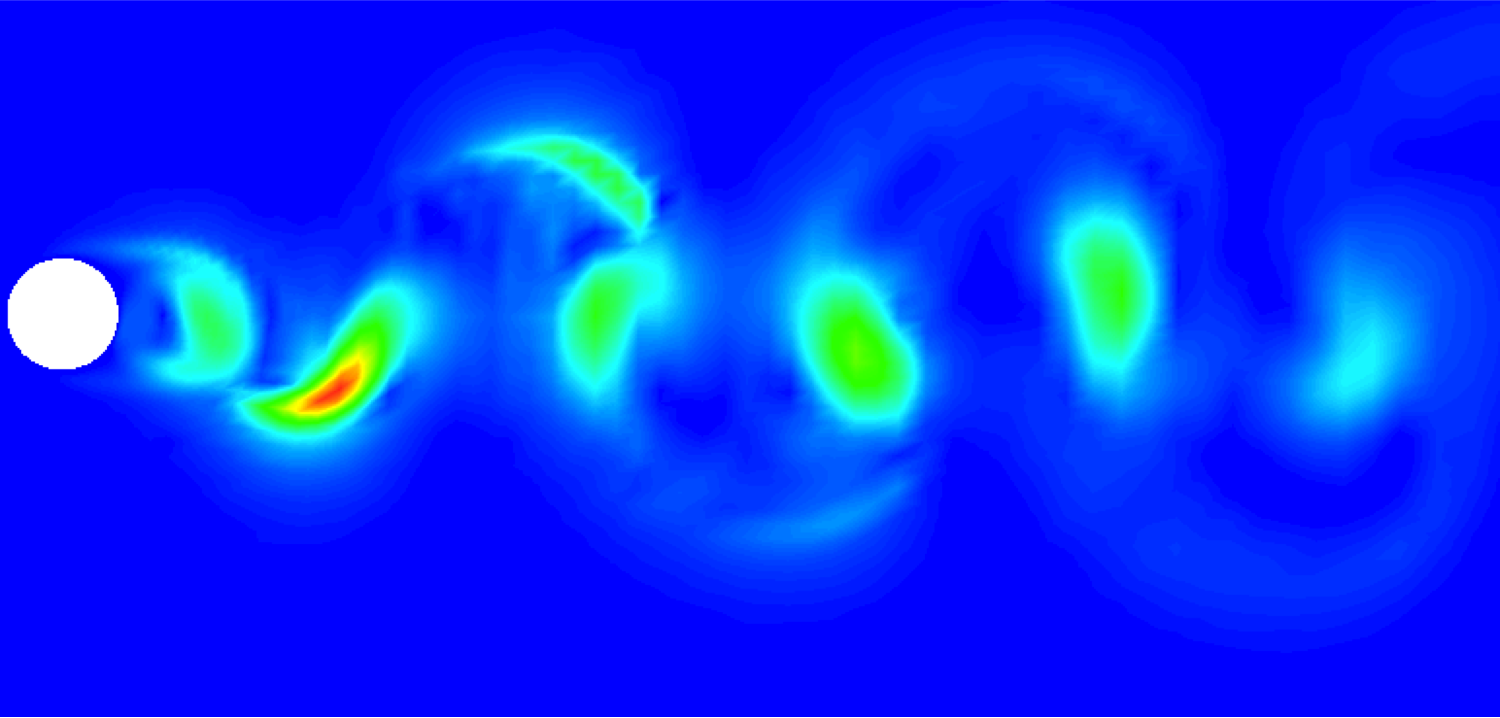
\includegraphics[width=1 \textwidth]{img/floquet}}
   \caption {}
\end{figure}

